\documentclass[a4paper, titlepage]{article}
\usepackage[T1]{fontenc}
\usepackage[utf8]{inputenc}
\usepackage[italian]{babel}
\usepackage{geometry}
\usepackage{graphicx}
\geometry{a4paper,top=3cm,bottom=3cm,left=3cm,right=3cm,%
heightrounded,bindingoffset=5mm}
% commenti su più righe
\usepackage{verbatim}
% librerie per tabelle
\usepackage{lscape}
\usepackage{longtable}
\usepackage{booktabs}
\usepackage[normalem]{ulem}
\useunder{\uline}{\ul}{}
\begin{document}

% Frontespizio
\begin{titlepage}
\centering
\vspace{5cm}
{\LARGE\bfseries Universit\`a degli Studi di Milano-Bicocca\par}
\vspace{1ex}
\hrule
\vspace{1ex}
Dipartimento di Informatica, Sistemistica e Comunicazione\\
Corso di Laurea Triennale in Informatica\\
\vspace{6cm}
Documentazione di progetto\\
\vspace{1cm}
{\Huge \bfseries \scshape Brew Day!\par}
\vspace{6cm}
\begin{tabular*}{\textwidth}{@{}l@{\extracolsep{\fill}}l@{}}
Alessia Calzari,   a.calzari@campus.unimib.it\\
Matricola: 844884\\
\\
Dario Gianotti,   d.gianotti2@campus.unimib.it\\
Matricola: 847052\\
\\
Andrea Provasi,   a.provasi2@campus.unimib.it\\
Matricola: 847015\\
\\
Riccardo Riva,   r.riva36@campus.unimib.it\\
Matricola: 844936
\end{tabular*}
\vspace{\fill}
\hrule
\vspace{1ex}
\centering
\textbf{Anno Accademico 2020-2021}
\end{titlepage}

% Sommario
\tableofcontents

\newpage
\section{Introduzione}
L'obiettivo di questo progetto è quello di sviluppare un'applicazione per i produttori di birra artigianale.\\
L'applicazione permette la registrazione degli utenti per salvare le proprie ricette, segnare l'elenco dei prodotti disponibili e la propria attrezzatura.\\
In questo modo l'utente potrà effettuare il login con le proprie credenziali per compiere diverse operazioni:
\begin{itemize}
    \item modificare il proprio account o eliminarlo;
    \item aggiungere una nuova ricetta (con prodotti, attrezzatura necessaria, preparazione e note) o eliminarne una dalla lista delle ricette;
    \item modificare una ricetta (aggiornare le note);
    \item aggiungere, rimuovere o modificare un attrezzo dalla lista delle attrezzature;
    \item aggiungere o rimuovere o modificare un prodotto alla lista dei prodotti;
    \item consultare la lista della spesa che contiene tutti i prodotti utilizzati e le loro quantità;
    \item scegliere la ricetta della birra da preparare ed indicarne la quantità, una volta selezionato questo gli ingredienti utilizzati saranno aggiunti alla lista della spesa;
    \item usare la funzionalità "Che birra faccio?" che mostrerà la ricetta che massimizza l'utilizzo degli ingredienti disponibili.
\end{itemize}

\newpage

\section{Avvio}
Per utilizzare questa applicazione non sono necessari particolari pre-requisiti, è sufficiente disporre di un computer.\\
Per avviare l'applicazione è necessario eseguire i seguenti passi:
\begin{enumerate}
    \item aprire la cartella "ProgettoBirra"
    \item selezionare e aprire la cartella "installer"
    \item selezionare ed eseguire il file "setup.exe"\\
    comparirà la finestra sottostante\\
    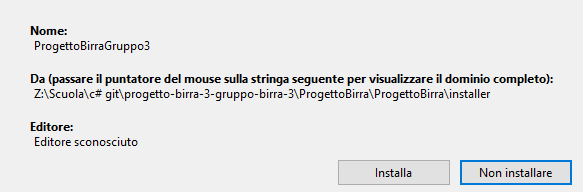
\includegraphics[scale=0.30]{Immagini/imgpsh_fullsize_anim.png}
    \item premere installa\\
    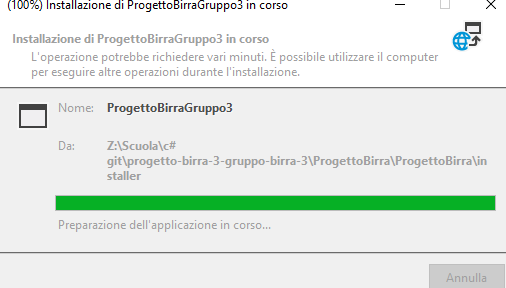
\includegraphics[scale=0.30]{Immagini/imgpsh_fullsize_anim (1).png}\\
    Al termine dell'installazione l'applicazione partirà autonomamente. Se così non dovesse succedere la si troverà nel menù applicazione.
\end{enumerate}

\section{Funzionamento}
\subsection{Registrazione}
All'avvio dell'applicazione l'utente si troverà davanti una finestra così strutturata:\\\\
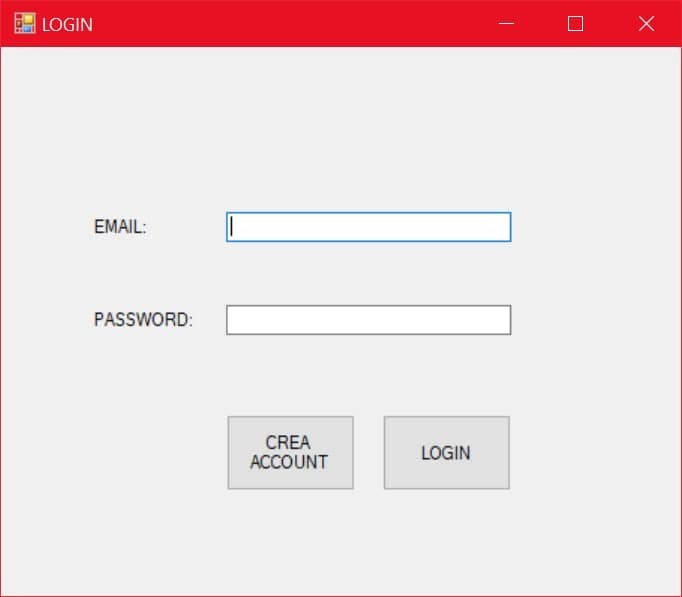
\includegraphics[scale=0.30]{Immagini/form/Form Login.jpg}
\\Per poter usare l'applicazione è necessario avere un account, quindi come primo passo l'utente dovrà premere sul bottone "CREA ACCOUNT":\\\\
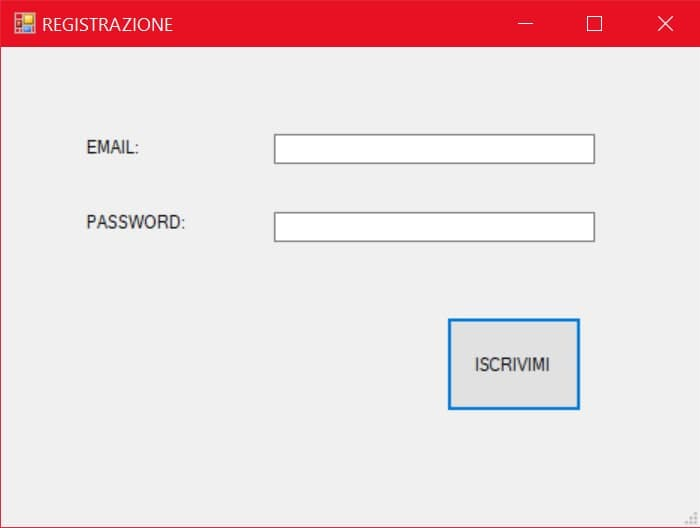
\includegraphics[scale=0.30]{Immagini/form/Form Registrazione.jpg}
\\Si troverà davanti a questa finestra e dopo aver compilato i campi procederà con l'iscrizione tramite il bottone "ISCRIVIMI".
Dopo di che verrà riportato alla schermata iniziale.
\newpage
\subsection{Login}
All'avvio dell'applicazione l'utente, già registrato, si troverà davanti la schermata mostrata come prima figura, potrà compilare i campi con email e password relativi al proprio account e premere sul bottone "LOGIN", si aprirà quindi la finestra del menu:\\\\
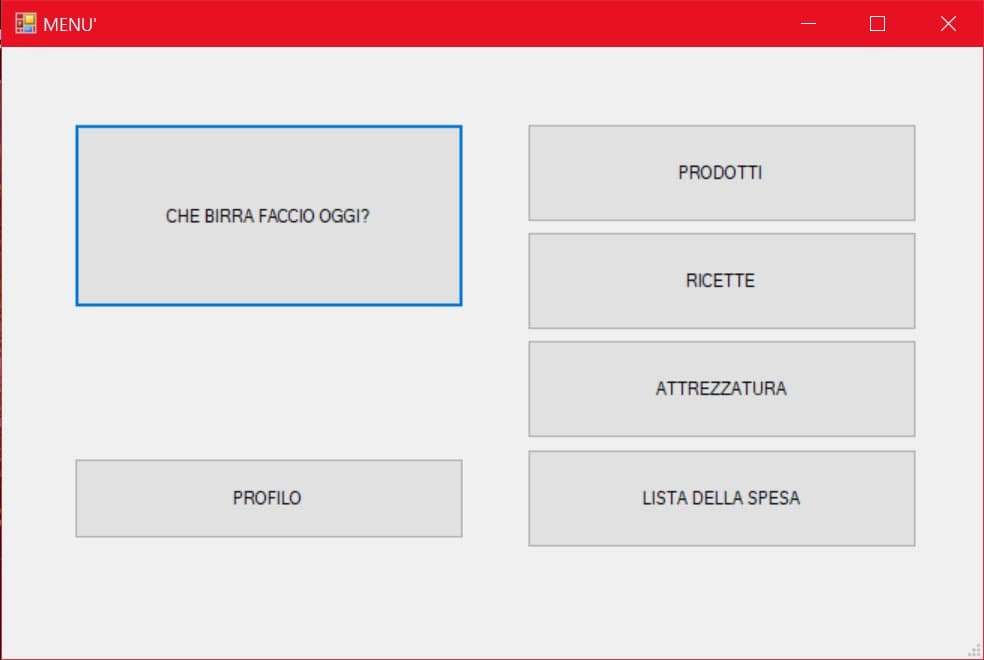
\includegraphics[scale=0.30]{Immagini/form/Form Menu.jpg}
\\e avrà la possibilità di scegliere tra diverse operazioni da compiere.
\subsection{Profilo}
Una volta all'interno dell'applicazione, dalla finestra del menù, l'utente potrà selezionare il bottone "PROFILO"\\\\
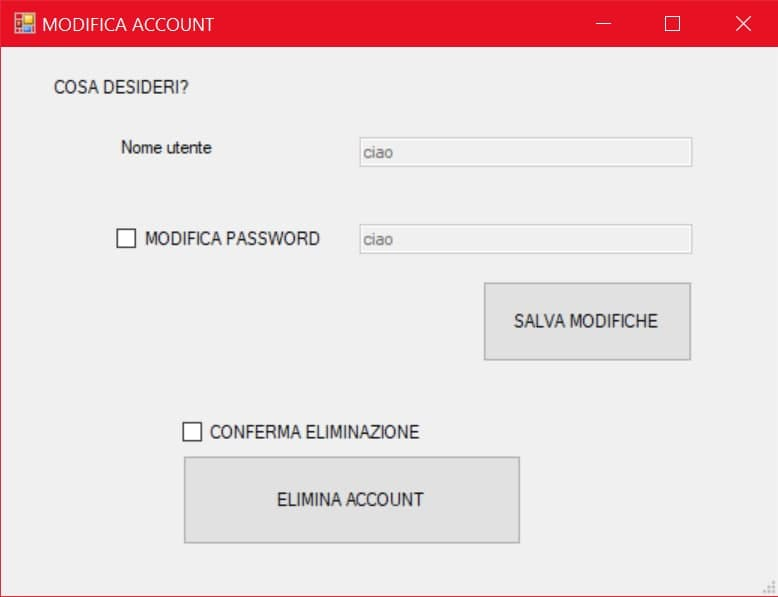
\includegraphics[scale=0.30]{Immagini/form/Form GestioneUtente.jpg}
\\Da questa finestra:
\begin{itemize}
    \item avrà la possibilità di modificare la propria password spuntando il box "MODIFICA PASSWORD" e premendo il bottone "SALVA MODIFICHE";
    \item potrà procedere con l'eliminazione del proprio account e di tutti i dati relativo ad esso spuntando il box "CONFERMA ELIMINAZIONE" e premendo il bottone "ELIMINA ACCOUNT".
\end{itemize} 
Al termine di queste operazioni l'utente verrà riportato alla schermata iniziale (immagine1)
\newpage
\subsection{Prodotti}
Una volta all'interno dell'applicazione, dalla finestra del menù, l'utente potrà premere il bottone "PRODOTTI"\\\\
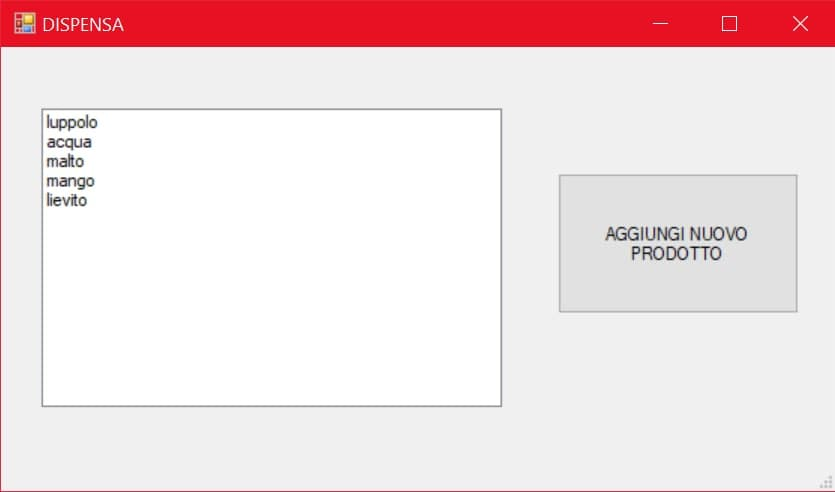
\includegraphics[scale=0.30]{Immagini/form/Form GestioneProdotti.jpg}
\\Da questa finestra potrà:
\begin{itemize}
    \item selezionare un prodotto presente nella lista schiacciandolo\\\\
    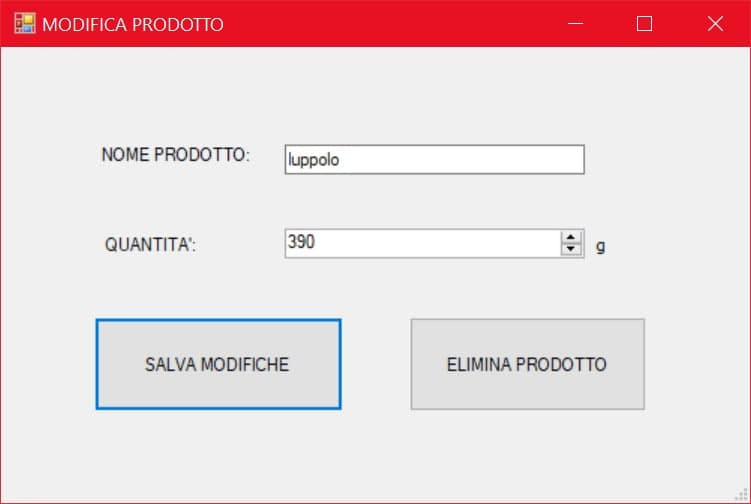
\includegraphics[scale=0.30]{Immagini/form/Form ModificaProd.jpg}
    \\Da questa finestra potrà scegliere:
        \subitem - di modificarne la quantità, scegliendo se inserire manualmente il numero oppure utilizzare le freccine, e premendo il bottone "SALVA MODIFICHE" salvare le modifiche apportate;
        \subitem - di eliminare il prodotto tramite il bottone "ELIMINA PRODOTTO".
    \item premere il bottone "AGGIUNGI NUOVO PRODOTTO"\\\\
    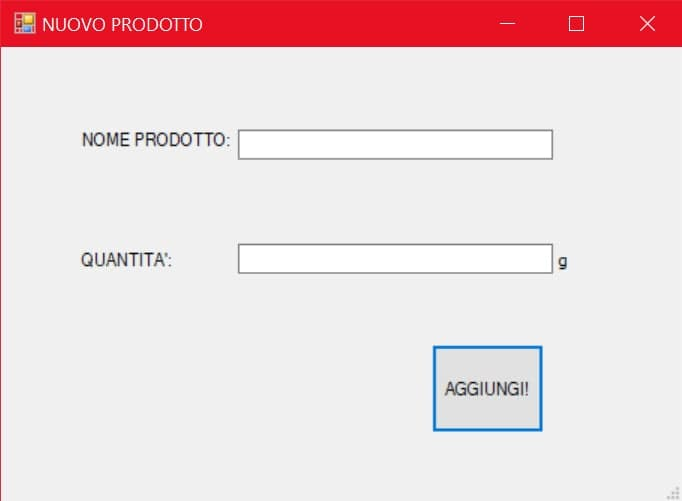
\includegraphics[scale=0.30]{Immagini/form/Form AggiuntaProd.jpg}
    \\Da questa finestra potrà inserire nome e quantità relativi al prodotto e tramite il bottone "AGGIUNGI!" aggiungerlo al database.
\end{itemize}
\newpage
\subsection{Ricette}
Una volta all'interno dell'applicazione, dalla finestra del menù, l'utente potrà premere il bottone "RICETTE"\\\\
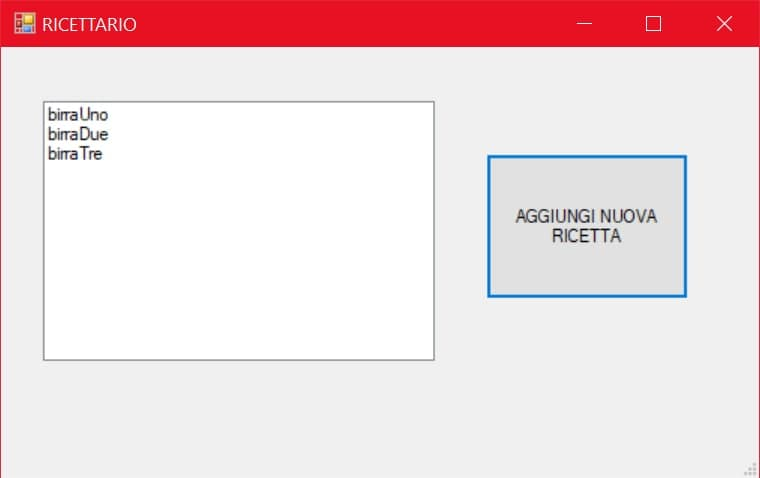
\includegraphics[scale=0.30]{Immagini/form/Form GestioneRicette.jpg}
\\Da questa finestra potrà:
\begin{itemize}
    \item premere il bottone "AGGIUNGI NUOVA RICETTA"\\\\
    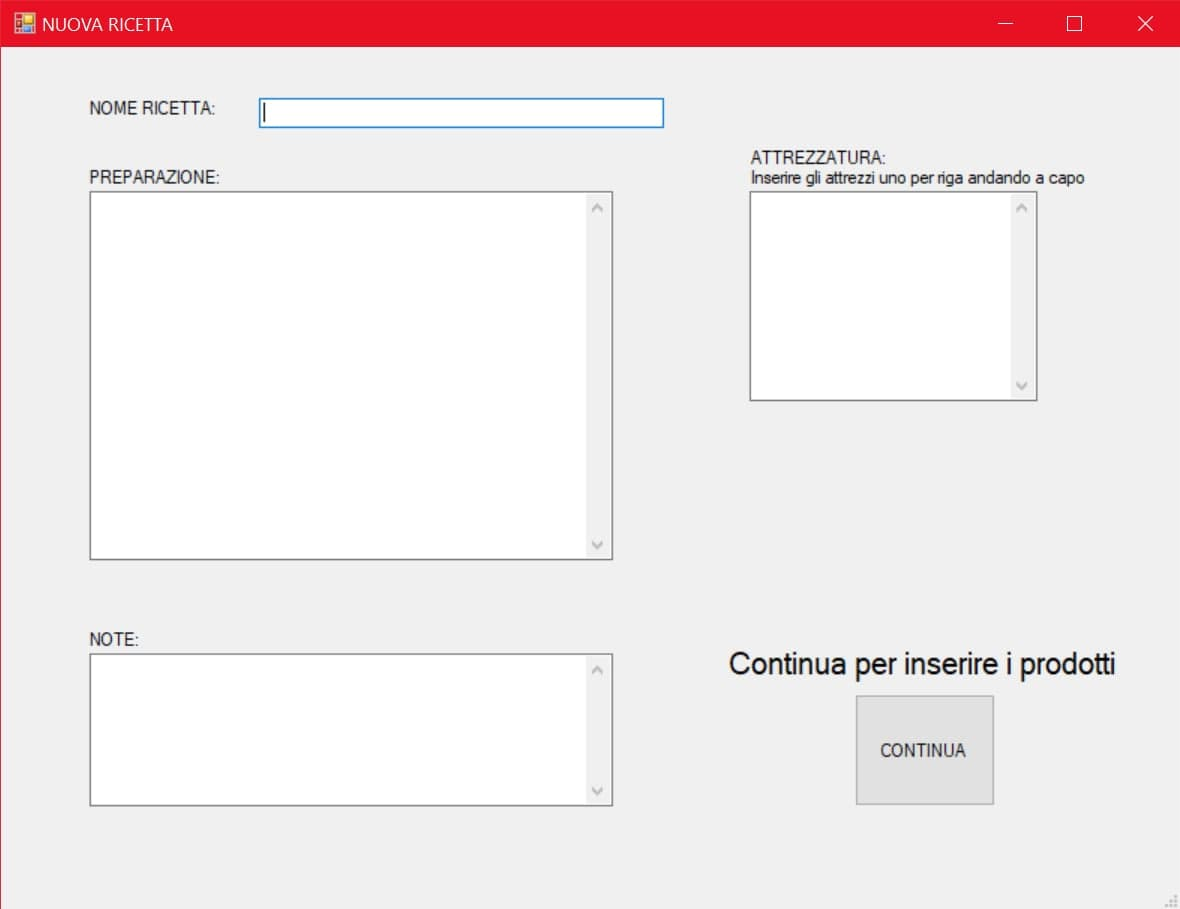
\includegraphics[scale=0.30]{Immagini/form/Form AggiungiRic.jpg}
    \\Da questa finestra potrà inserire nome, preparazione, attrezzi e premere "CONTINUA" per inserire i prodotti relativi alla ricetta salvandoli tramite il bottone "SALVA PRODOTTO"\\\\
    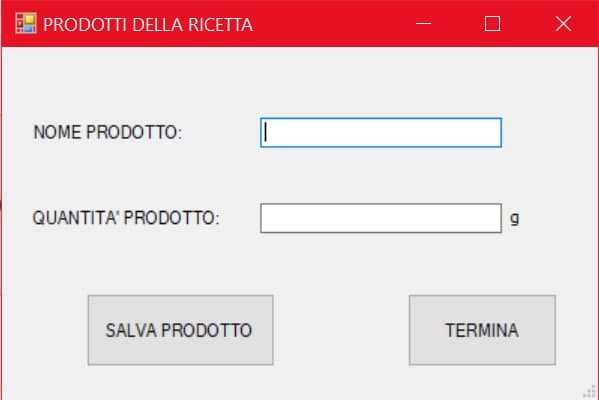
\includegraphics[scale=0.30]{Immagini/form/Form AggiungiProdottiRicetta.jpg}
    \\e per terminare l'inserimento dei prodotti e ultimare il salvataggio della ricetta premerà "TERMINA";
    \newpage
    \item selezionare una ricetta presente nella lista schiacciandolo\\\\
    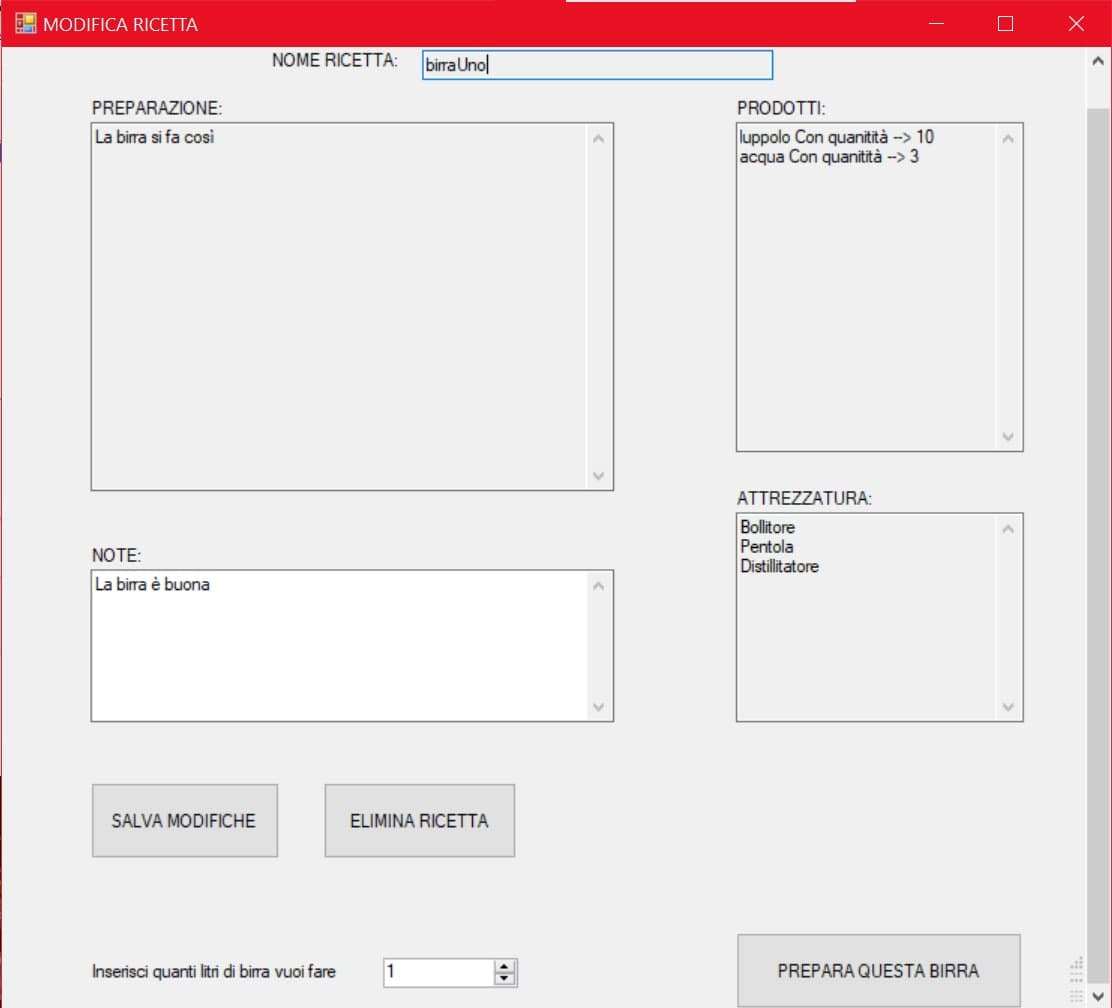
\includegraphics[scale=0.30]{Immagini/form/Form Ricetta.jpg}
    \\Da questa finestra potrà scegliere:
        \subitem - di modificarne le note scrivendo nello spazio apposito e premendo il bottone "SALVA MODIFICHE";
        \subitem - di eliminare la ricetta tramite il bottone "ELIMINA PRODOTTO";
        \subitem - di preparare una birra inserendo nello spazio apposito il numero di litri (manualmente o tramite le freccine) e premendo "PREPARA QUESTA BIRRA"
\end{itemize}
\subsection{Attrezzatura}
Una volta all'interno dell'applicazione, dalla finestra del menù, l'utente potrà premere il bottone "ATTREZZATURA"\\\\
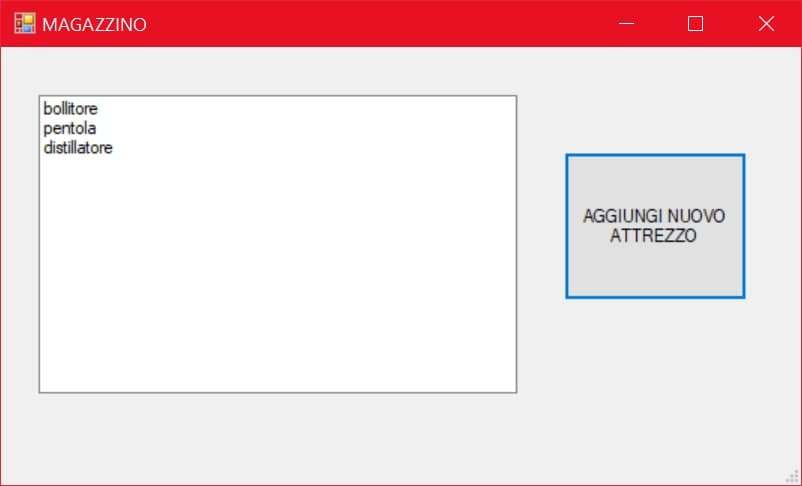
\includegraphics[scale=0.30]{Immagini/form/Form GestioneAttrezzatura.jpg}
\\Da questa finestra potrà:
\begin{itemize}
    \item selezionare un attrezzo presente nella lista schiacciandolo\\\\
    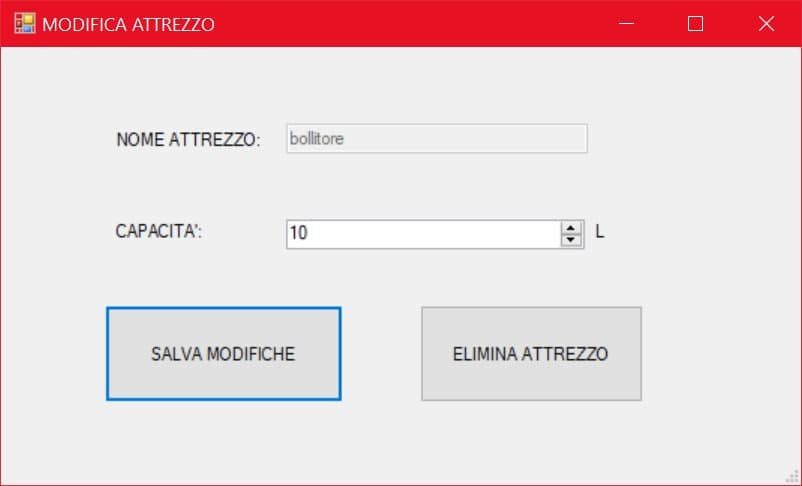
\includegraphics[scale=0.30]{Immagini/form/Form ModificaAtt.jpg}
    \\Da questa finestra potrà scegliere:
        \subitem - di modificarne la capacità, scegliendo se inserire manualmente il numero oppure utilizzare le freccine, e premendo il bottone "SALVA MODIFICHE" salvare le modifiche apportate;
        \subitem - di eliminare il prodotto tramite il bottone "ELIMINA ATTREZZO".
    \item premere il bottone "AGGIUNGI NUOVO ATTREZZO"\\
    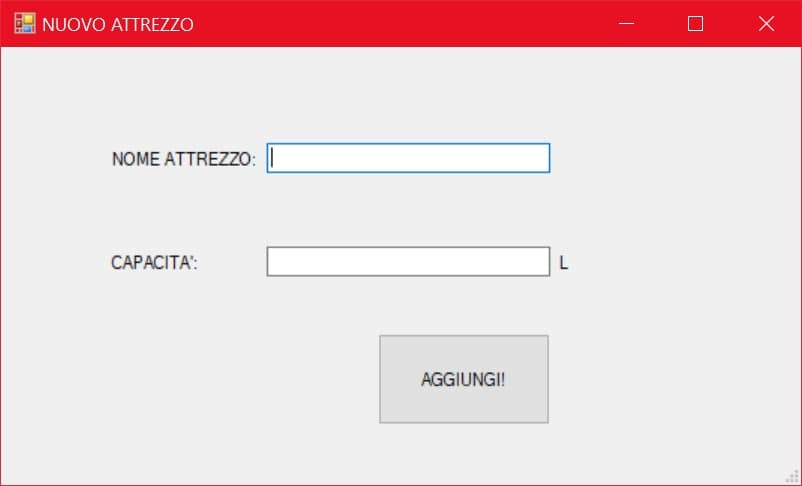
\includegraphics[scale=0.30]{Immagini/form/Form AggiuntaAtt.jpg}
    \\da questa finestra potrà inserire nome e quantità relativi all'attrezzo e tramite il bottone "AGGIUNGI!" aggiungerlo al database.
\end{itemize}
\subsection{Lista della spesa}
Una volta all'interno dell'applicazione, dalla finestra del menù, l'utente potrà premere il bottone "LISTA DELLA SPESA"\\\\\
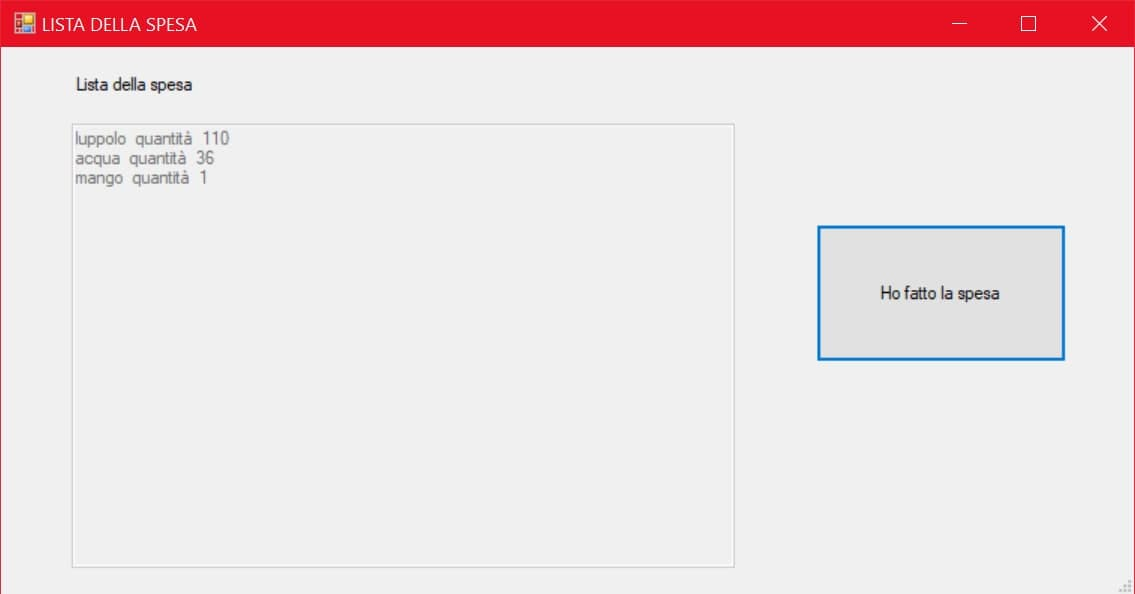
\includegraphics[scale=0.30]{Immagini/form/Form ListaSpesa.jpg}
\\Da questa finestra potrà visualizzare la lista dei prodotti mancanti con le relative quantità e cancellarla tramite il bottone "HO FATTO LA SPESA".
\subsection{"Che birra faccio oggi?"}
Una volta all'interno dell'applicazione, dalla finestra del menù, l'utente potrà premere il bottone "CHE BIRRA FACCIO OGGI?" che gli restituirà una finestra con il nome della birra e la quantità massima che è possibile preparare. La birra visualizzata sarà quella di cui è possibile preparare la maggior quantità considerando i prodotti presenti nel database.

\newpage
\section{Analisi}
\subsection{Diagramma dei casi d'uso}
Sono stati identificati otto casi d'uso che di seguito vengono illustrati nella forma dettagliata.
\vphantom{}
\subsection{Casi d'uso}
\vphantom{}
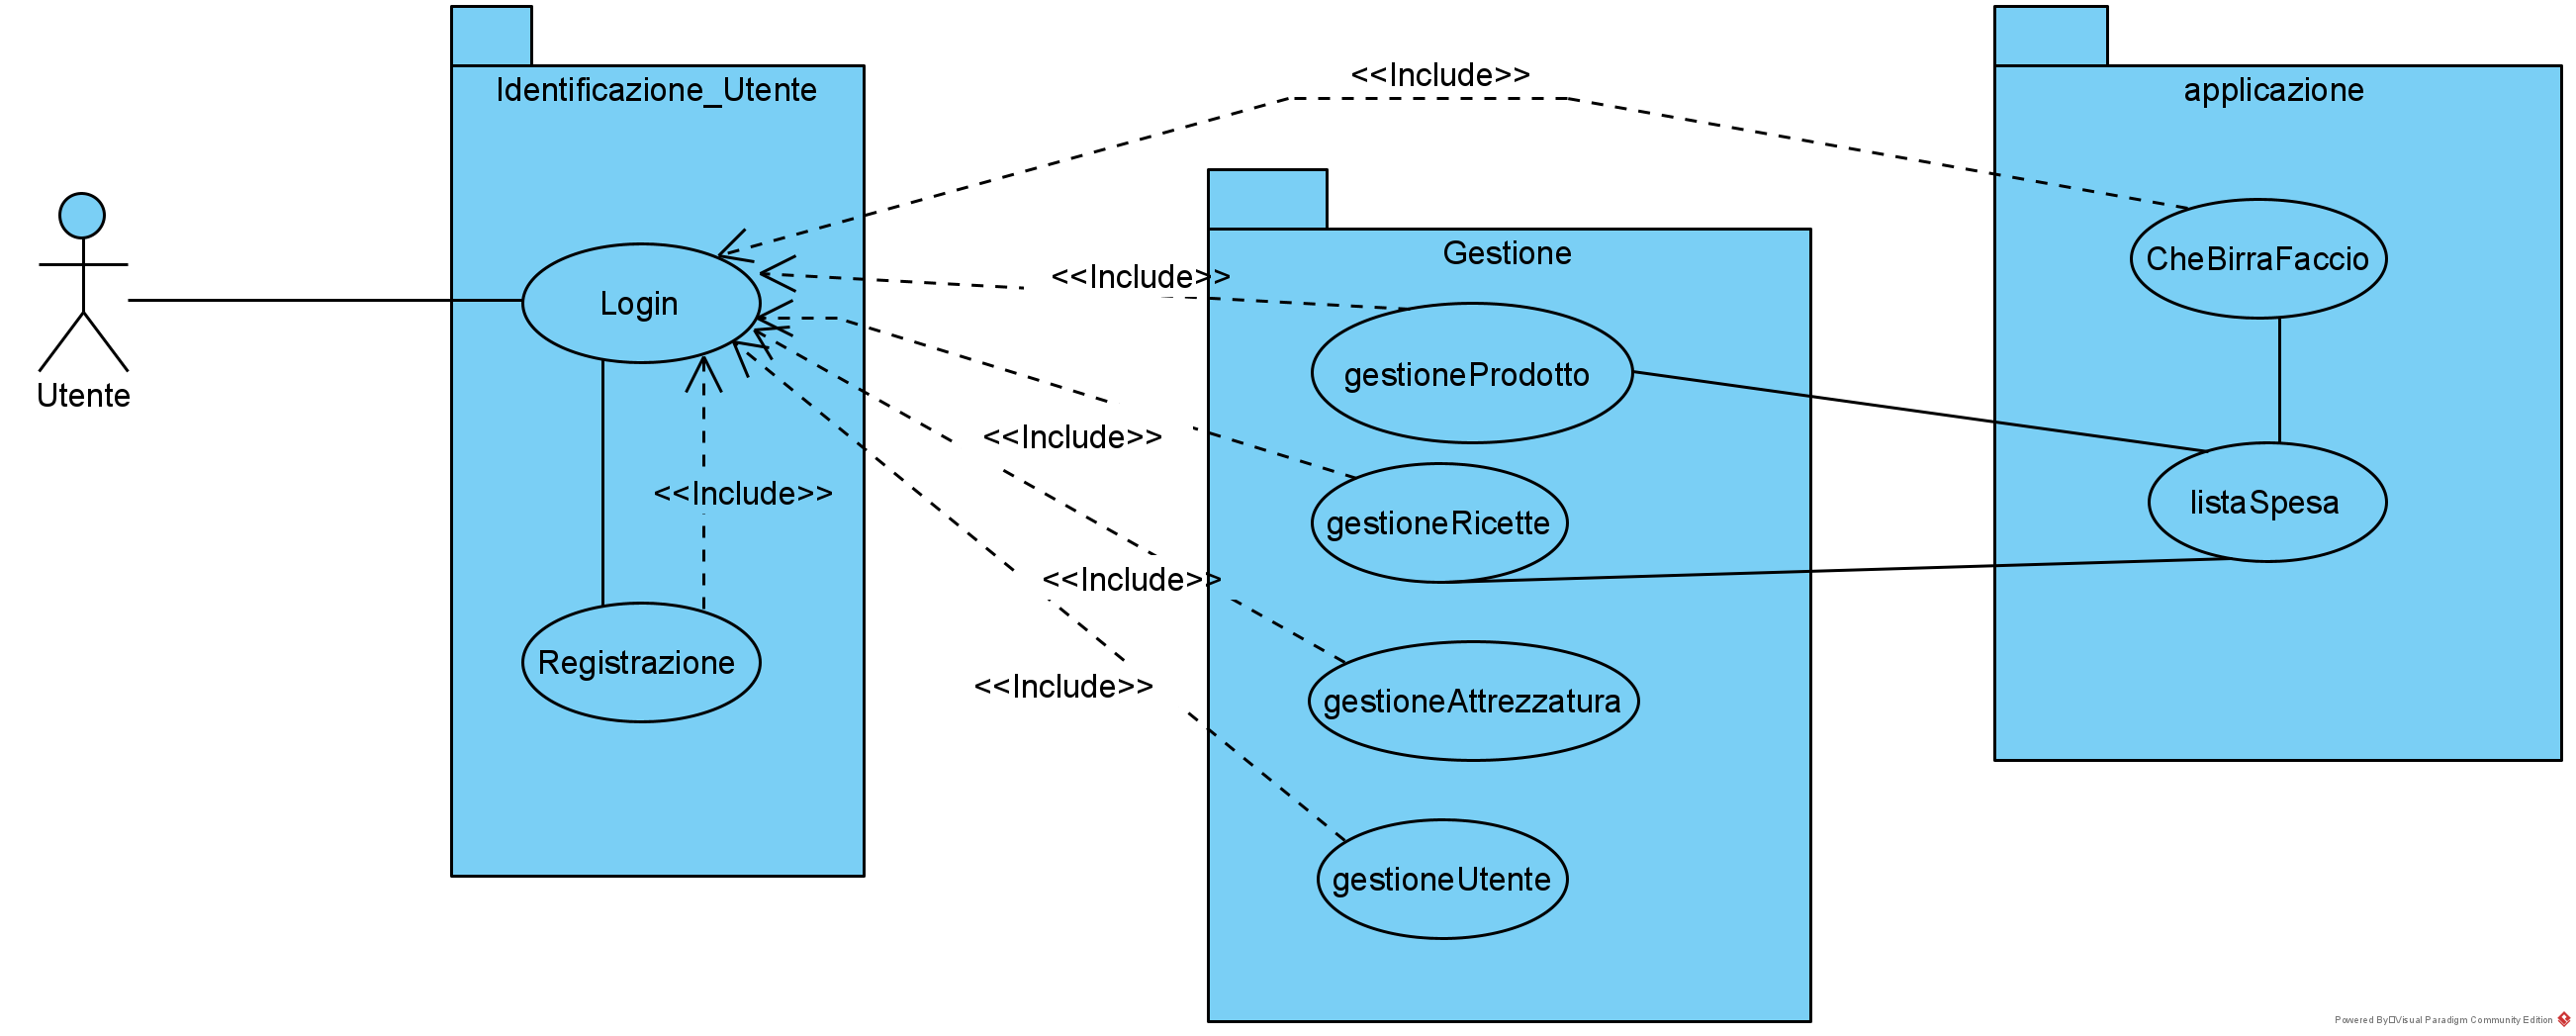
\includegraphics[scale=0.65]{Immagini/Use Case Diagram_Brew Day!.png}
\vphantom{}
\subsubsection{Login}
\begin{longtable}{p{6cm}p{7cm}}\toprule
    NOME & Login\\\midrule
    PORTATA & Brew Day!\\\midrule
    LIVELLO & Gestione di ricette di birre artigianali\\\midrule
    ATTORE PRIMARIO & Utente\\\midrule
    PARTI INTERESSATE E INTERESSI & L’attore Utente vuole accedere al sito “Brew Day!” inserendo le proprie credenziali\\\midrule
    PRE-CONDIZIONI & L’attore Utente deve aver effettuato la registrazione\\\midrule
    GARANZIA DI SUCCESSO & L’attore Utente riesce ad accedere al sito di “Brew Day!”\\\midrule
    SCENARIO PRINCIPALE DI
    & 1) il sistema visualizza la schermata login\\
    SUCCESSO & 2) l’utente inserisce le credenziali\\
    & 3) il sistema verifica la correttezza
    dei dati sul database\\\midrule
    ESTENSIONI &
    3.1) in caso di dati corretti viene effettuato il login\\
    & 3.2) in caso di dati errati il sistema
    visualizza un messaggio di errore\\\midrule
    REQUISITI SPECIALI & Nessuno \\\midrule
    ELENCO VARIABILI TECNOLOGICHE & Database\\\midrule
    FREQUENZA DI RIPETIZIONE & Più volte al giorno\\\midrule
    VARIE & Nessuna\\\bottomrule
\end{longtable}
\vphantom{}
\subsubsection{Registrazione}
\begin{longtable}{p{6cm}p{7cm}}\toprule
    NOME & Registrazione\\\midrule
    PORTATA & Brew Day!\\\midrule
    LIVELLO & Gestione di ricette di birra artigianali\\\midrule
    ATTORE PRIMARIO & Utente\\\midrule
    PARTI INTERESSATE E INTERESSI & L’attore Utente vuole registrarsi al sito di “Brew Day!" inserendo e-mail e password\\\midrule
    PRE-CONDIZIONI & Nessuna\\\midrule
    GARANZIA DI SUCCESSO & L’attore Utente viene registrato\\\midrule
    SCENARIO PRINCIPALE DI
    & 1) l’utente preme su "Crea Account"\\
    SUCCESSO & 2) il sistema visualizza la schermata di registrazione (e-mail e password)\\
    & 3) l’utente inserisce i propri dati\\
    & 4) il sistema   verifica la correttezza dei dati inseriti\\\midrule
    ESTENSIONI
    & 4.1) in caso di dati corretti essi vengono inseriti
    nel database ed il sistema visualizza un messaggio di successo\\
    & 4.2) in caso di dati errati viene visualizzato un messaggio di errore ed il cliente può reinserire i dati\\\midrule
    REQUISITI SPECIALI & Nessuno\\\midrule
    ELENCO VARIABILI TECNOLOGICHE & Database\\\midrule
    FREQUENZA DI RIPETIZIONE & Una volta per utente\\\midrule
    VARIE & Nessuna\\\bottomrule                                
\end{longtable}
\newpage
\vphantom{}
\subsubsection{gestioneUtente}
\begin{longtable}{p{6cm}p{7cm}}\toprule
    NOME & gestioneUtente\\\midrule
    PORTATA & Brew Day!\\\midrule
    LIVELLO & Gestione di ricette di birra artigianali\\\midrule
    ATTORE PRIMARIO & Utente\\\midrule
    PARTI INTERESSATE E INTERESSI & L’attore Utente vuole visualizzare il proprio profilo, modificare informazioni o eliminarlo\\\midrule
    PRE-CONDIZIONI & Login\\\midrule
    GARANZIA DI SUCCESSO & L’attore Utente riesce a visualizzare il proprio profilo, modificare informazioni o eliminarlo\\\midrule
    SCENARIO PRINCIPALE DI
    & 1) l’utente seleziona la voce "Profilo"\\
    SUCCESSO & 2) il sistema restituisce la schermata con i dati del profilo\\
    & 3.1) l’utente seleziona “modifica password” e scrive la nuova password\\
    & 3.2) l’utente seleziona “elimina profilo”\\
    & 4.1) l'utente preme “salva modifiche”\\
    & 4.2) il sistema visualizza una schermata di conferma eliminazione\\
    & 5.2) l’utente conferma\\
    & 5.1) il sistema salva il nuovi dati nel database e restituisce un messaggio di conferma\\
    & 6.2) il sistema elimina i dati relativi dal database e restituisce un messaggio di conferma\\\midrule
    ESTENSIONI
    & 5.1.1) se il profilo non viene salvato correttamente, il sistema restituisce un messaggio di errore\\
    & 6.2.1) se il profilo non viene eliminato correttamente, il sistema restituisce un messaggio di errore\\\midrule
    REQUISITI SPECIALI & Nessuno\\\midrule
    ELENCO VARIABILI TECNOLOGICHE & Database\\\midrule
    FREQUENZA DI RIPETIZIONE & Più volte al giorno\\\midrule
    VARIE & Nessuna\\\bottomrule
\end{longtable}
\vphantom{}
\newpage
\subsubsection{gestioneProdotto}
\begin{longtable}{p{6cm}p{7cm}}\toprule
    NOME & gestioneProdotto\\\midrule
    PORTATA & Brew Day!\\\midrule
    LIVELLO & Gestione di ricette di birra artigianali\\\midrule
    ATTORE PRIMARIO & Utente\\\midrule
    PARTI INTERESSATE E INTERESSI & L’attore Utente vuole visualizzare la lista dei prodotti, modificare, aggiungere o rimuovere i prodotti che ha in casa\\\midrule
    PRE-CONDIZIONI & Login\\\midrule
    GARANZIA DI SUCCESSO &  L’attore Utente riesce a visualizzare la lista dei prodotti, modificare, aggiungere o rimuovere i prodotti che ha in casa\\\midrule
    SCENARIO PRINCIPALE DI
    & 1) l’utente seleziona la voce prodotti\\
    SUCCESSO & 2) il sistema restituisce la lista dei prodotti\\
    & 3.1) l’utente seleziona “aggiungi prodotto”\\
    & 3.2) l’utente seleziona il prodotto desiderato dalla lista\\
    & 4.1) il sistema restituisce la schermata per aggiungere il prodotto\\
    & 4.2) il sistema restituisce la schermata del prodotto\\
    & 5.1) l’utente inserisce i dati del prodotto e salva\\
    & 5.2) l’utente modifica i dati che desidera e preme su “salva”\\
    & 5.3) l’utente preme su “elimina”\\
    & 6.1) il sistema salva i nuovi dati nel database e restituisce un messaggio di conferma\\
    & 6.2) il sistema salva i nuovi dati nel database e restituisce un messaggio di conferma\\
    & 6.3) il sistema elimina i dati relativi al prodotto dal database e restituisce un messaggio di conferma\\\midrule
    ESTENSIONI
    & 6.1.1) se il prodotto non viene salvato correttamente, il sistema restituisce un messaggio di errore\\
    & 6.2.1) se il prodotto non viene salvato correttamente, il sistema restituisce un messaggio di errore\\
    & 6.3.1) se il prodotto non viene eliminato correttamente, il sistema restituisce un messaggio di errore \\\midrule
    REQUISITI SPECIALI & Nessuno\\\midrule
    ELENCO VARIABILI TECNOLOGICHE & Database\\\midrule
    FREQUENZA DI RIPETIZIONE & Più volte al giorno\\\midrule
    VARIE & Nessuna\\\bottomrule
\end{longtable}
\vphantom{}
\subsubsection{gestioneAttrezzatura}
\begin{longtable}{p{6cm}p{7cm}}\toprule
    NOME & gestioneAttrezzatura\\\midrule
    PORTATA & Brew Day!\\\midrule
    LIVELLO & Gestione di ricette di birra artigianali\\\midrule
    ATTORE PRIMARIO & Utente\\\midrule
    PARTI INTERESSATE E INTERESSI &
    L’attore Utente vuole visualizzare la lista dell’attrezzatura, aggiungere o rimuovere attrezzatura che ha in casa \\\midrule
    PRE-CONDIZIONI & Login\\\midrule
    GARANZIA DI SUCCESSO & L’attore Utente riesce a visualizzare la lista dell’attrezzatura, aggiungere o rimuovere
    attrezzatura che ha in casa\\\midrule
    SCENARIO PRINCIPALE DI
    & 1) l’utente seleziona la voce attrezzatura\\
    SUCCESSO & 2) il sistema restituisce la lista dell’attrezzatura\\
    & 3.1) l’utente seleziona “aggiungi attrezzo”\\
    & 3.2) l’utente seleziona l'attrezzo desiderato dalla lista\\
    & 4.1) il sistema restituisce la schermata per aggiungere l'attrezzo\\
    & 4.2) il sistema restituisce la schermata dell'attrezzo\\
    & 5.1) l’utente inserisce i dati dell'attrezzo e salva\\
    & 5.2) l’utente modifica i dati che desidera e preme su “salva”\\
    & 5.3) l’utente preme su “elimina”\\
    & 6.1) il sistema salva i nuovi dati nel database e restituisce un messaggio di conferma\\
    & 6.2) il sistema salva i nuovi dati nel database e restituisce un messaggio di conferma\\
    & 6.3) il sistema elimina i dati relativi all'attrezzo dal database e restituisce un messaggio di conferma\\\midrule
    ESTENSIONI
    & 6.1.1) se l'attrezzo non viene salvato correttamente, il sistema restituisce un messaggio di errore\\
    & 6.2.1) se l'attrezzo non viene salvato correttamente, il sistema restituisce un messaggio di errore\\
    & 6.3.1) se l'attrezzo non viene eliminato correttamente, il sistema restituisce un messaggio di errore \\\midrule
    REQUISITI SPECIALI & Nessuno\\\midrule
    ELENCO VARIABILI TECNOLOGICHE & Database\\\midrule
    FREQUENZA DI RIPETIZIONE & Più volte al giorno\\\midrule
    VARIE & Nessuna\\\bottomrule
\end{longtable}
\vphantom{}
\subsubsection{gestioneRicette}
\begin{longtable}{p{6cm}p{7cm}}\toprule
    NOME & gestioneRicette\\\midrule
    PORTATA & Brew Day!\\\midrule
    LIVELLO & Gestione di ricette di birra artigianali\\\midrule
    ATTORE PRIMARIO & Utente\\\midrule
    PARTI INTERESSATE E INTERESSI &
    L’attore Utente vuole visualizzare la lista delle ricette, modificare, aggiungere o rimuovere i prodotti che ha in casa \\\midrule
    PRE-CONDIZIONI & Login\\\midrule
    GARANZIA DI SUCCESSO & L’attore Utente riesce a visualizzare la lista delle ricette, modificare, aggiungere o rimuovere i prodotti che ha in casa \\\midrule
    SCENARIO PRINCIPALE DI
    & 1) l’utente seleziona la voce ricette\\
    SUCCESSO & 2) il sistema restituisce la lista delle ricette\\
    & 3.1) l’utente seleziona “aggiungi ricetta”\\
    & 3.2) l’utente seleziona la ricetta desiderata dalla lista\\
    & 4.1) il sistema restituisce la schermata per aggiungere la ricetta\\
    & 4.2) il sistema restituisce la schermata della ricetta\\
    & 5.1) l’utente inserisce i dati della ricetta e salva\\
    & 5.2) l’utente modifica i dati che desidera e preme su “salva”\\
    & 5.3) l’utente preme su “elimina ricetta”\\
    & 5.4) l'utente seleziona la quantità da produrre e preme su "prepara birra"\\
    & 6.2) il sistema salva i nuovi dati nel database e restituisce un messaggio di conferma\\
    & 6.3) il sistema elimina i dati relativi alla ricetta dal database e restituisce un messaggio di conferma\\
    & 6.4) il sistema sposta dalla lista dei prodotti alla lista della spesa la quantità di prodotti utilizzata per la preparazione della ricetta\\\midrule
    ESTENSIONI
    & 5.1.1) se la ricetta non viene salvata correttamente, il sistema restituisce un messaggio di errore\\
    & 6.2.1) se la ricetta non viene salvata correttamente, il sistema restituisce un messaggio di errore\\
    & 6.3.1) se la ricetta non viene eliminata correttamente, il sistema restituisce un messaggio di errore \\
    & 6.4.1) se l'utente non ha quantità sufficienti di prodotti per la preparazione, il sistema restituisce un messaggio di errore\\\midrule
    REQUISITI SPECIALI & Nessuno\\\midrule
    ELENCO VARIABILI TECNOLOGICHE & Database\\\midrule
    FREQUENZA DI RIPETIZIONE & Più volte al giorno\\\midrule
    VARIE & Nessuna\\\bottomrule
\end{longtable}
\vphantom{}
\subsubsection{listaSpesa}
\begin{longtable}{p{6cm}p{7cm}}\toprule
    NOME & listaSpesa\\\midrule
    PORTATA & Brew Day!\\\midrule
    LIVELLO & Gestione di ricette di birra artigianali\\\midrule
    ATTORE PRIMARIO & Utente\\\midrule
    PARTI INTERESSATE E INTERESSI & L’attore Utente vuole visualizzare la lista dei prodotti da comprare\\\midrule
    PRE-CONDIZIONI & Login\\\midrule
    GARANZIA DI SUCCESSO & L’attore Utente riesce a  visualizzare la lista dei prodotti da comprare\\\midrule
    SCENARIO PRINCIPALE DI
    & 1) l'utente preme su "lista della spesa"\\
    SUCCESSO & 2) il sistema restituisce la lista della spesa\\
    & 3) l’utente preme su “ho fatto la spesa”\\
    & 4) il sistema cancella la lista della spesa\\\midrule
    ESTENSIONI & Nessuna\\\midrule
    REQUISITI SPECIALI & Nessuno\\\midrule
    ELENCO VARIABILI TECNOLOGICHE & Database\\\midrule
    FREQUENZA DI RIPETIZIONE & Più volte al giorno\\\midrule
    VARIE & Nessuna\\\bottomrule
\end{longtable}
\vphantom{}
\newpage
\subsubsection{CheBirraFaccio}
\begin{longtable}{p{6cm}p{7cm}}\toprule
    NOME & CheBirraFaccio\\\midrule
    PORTATA & Brew Day!\\\midrule
    LIVELLO & Gestione di ricette di birra artigianali\\\midrule
    ATTORE PRIMARIO & Utente\\\midrule
    PARTI INTERESSATE E INTERESSI &
    L’attore Utente vuole un consiglio sulla birra da preparare\\\midrule
    PRE-CONDIZIONI & Login\\\midrule
    GARANZIA DI SUCCESSO &L’attore Utente riesce ad avere la ricetta della birra da preparare che massimizza l’uso dei prodotti disponibili\\\midrule
    SCENARIO PRINCIPALE DI
    & 1) l’utente preme su “Che birra faccio oggi?”\\
    SUCCESSO & 2) il sistema calcola che birra fare in base alla quantità di prodotti e alle ricette presenti nel database\\
    & 3) il sistema restituisce un messaggio con il nome della ricetta e il numero massimo di litri che si possono produrre\\
    ESTENSIONI
    & 3.1) se l'utente non ha abbastanza prodotti per produrre alcuna ricetta presente nel database il sistema restituisce un messaggio di errore\\\midrule
    REQUISITI SPECIALI & Nessuno\\\midrule
    ELENCO VARIABILI TECNOLOGICHE & Database\\\midrule
    FREQUENZA DI RIPETIZIONE & Più volte al giorno\\\midrule
    VARIE & Nessuna \\\bottomrule
\end{longtable}

%%\begin{tabular}[c]{@{}l@{}} \end{tabular}\\\midrule
\newpage
\subsection{Diagramma delle classi a livello di Dominio}
In questo diagramma sono presenti le classi implementate con i relativi attributi e viene mostrato come interagiscono tra loro.\\\\
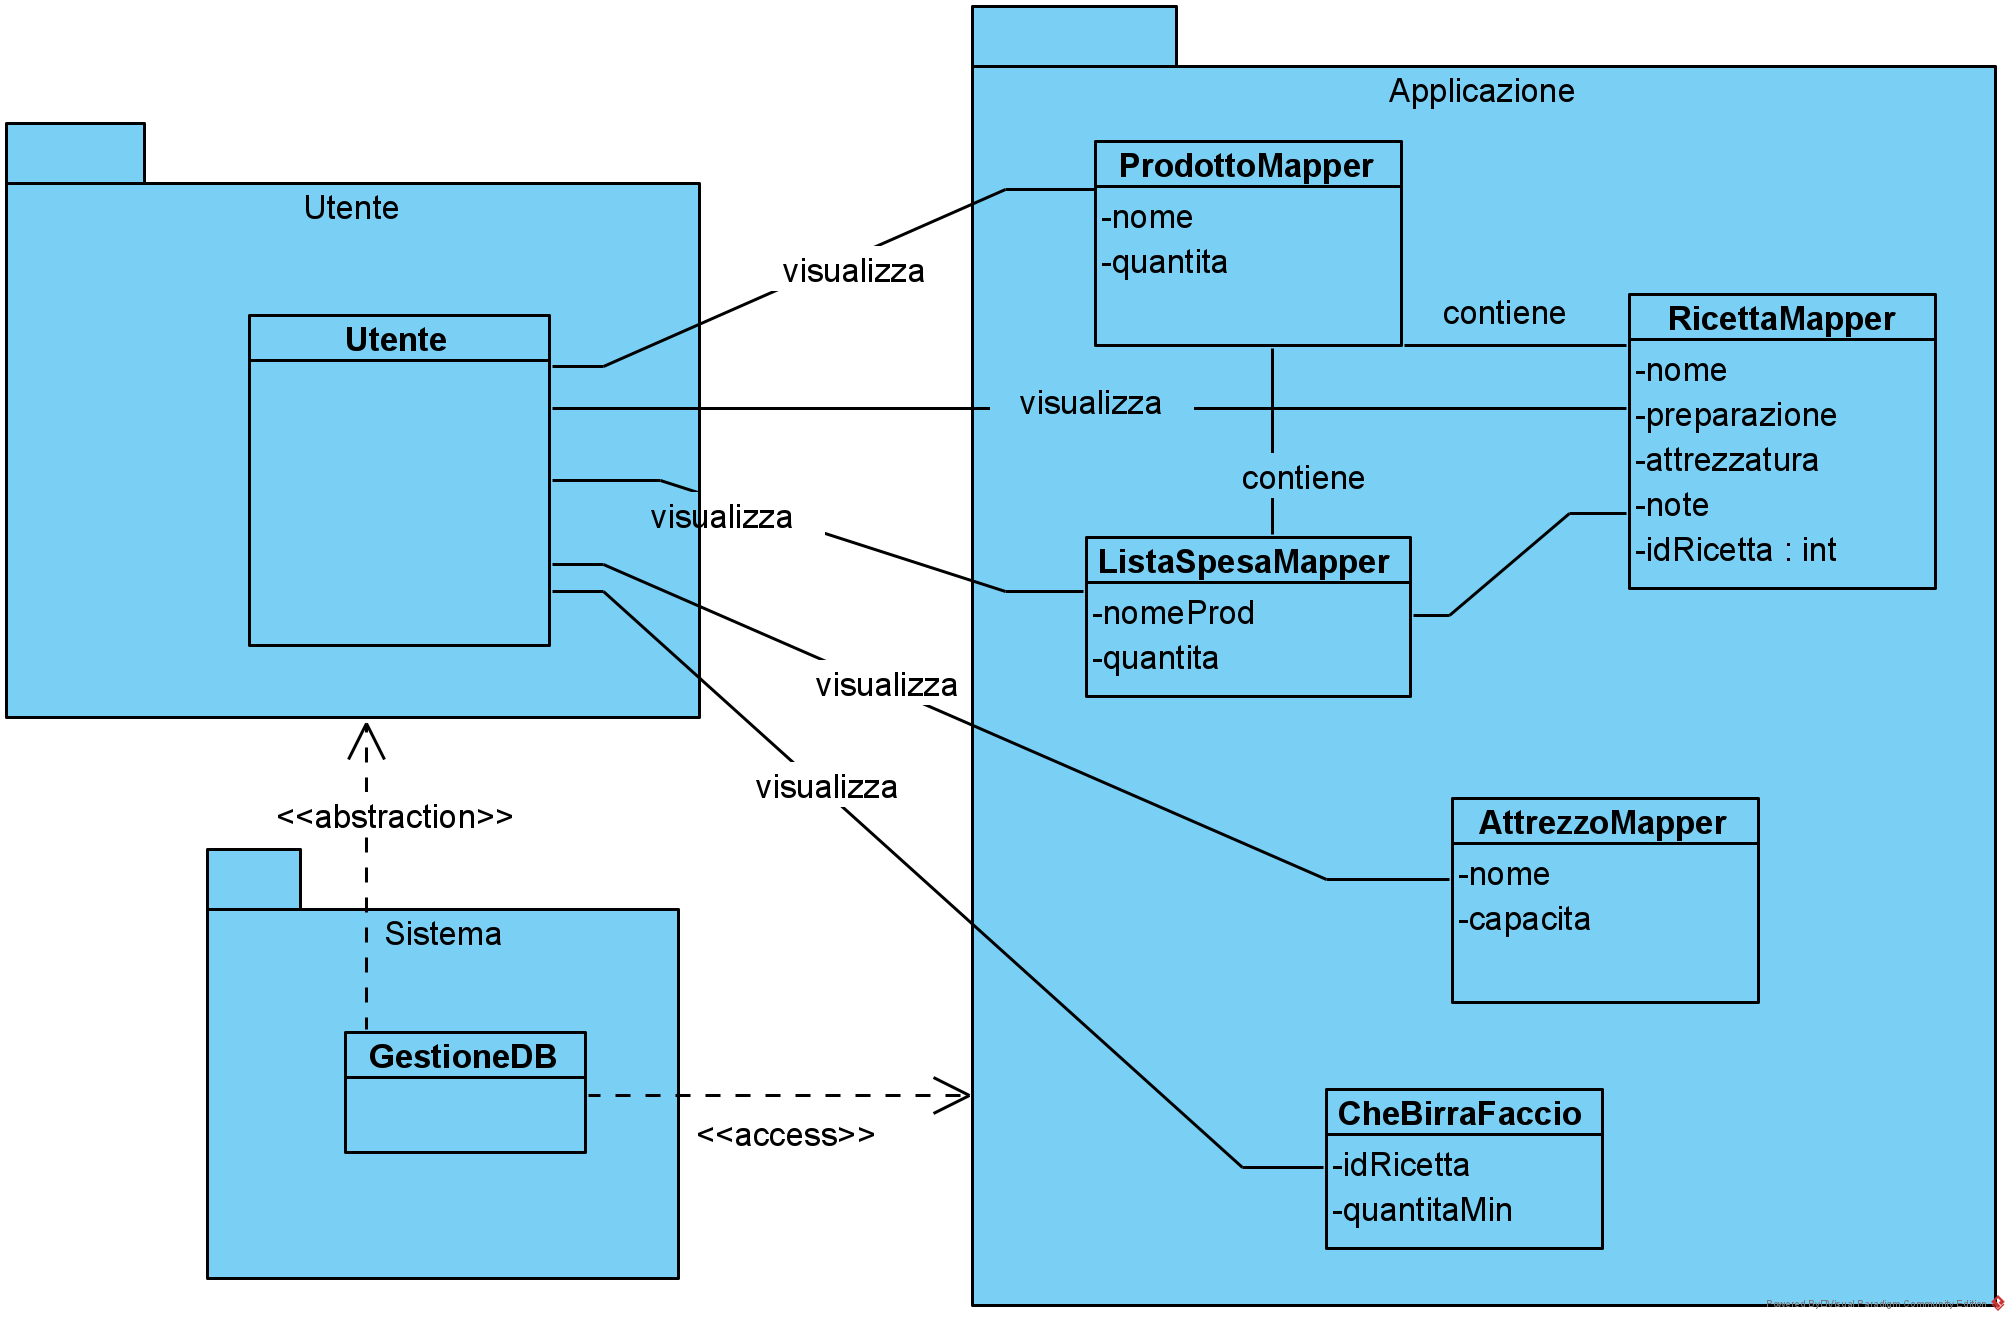
\includegraphics[scale=0.50]{Immagini/Domain Model_Brew Day!_definitivo.png}
\subsection{Diagramma delle classi a livello di Progettazione}
In questo diagramma sono presenti tutte le classi implementate con i relativi attributi e metodi e viene mostrato come interagiscono tra loro.\\\\
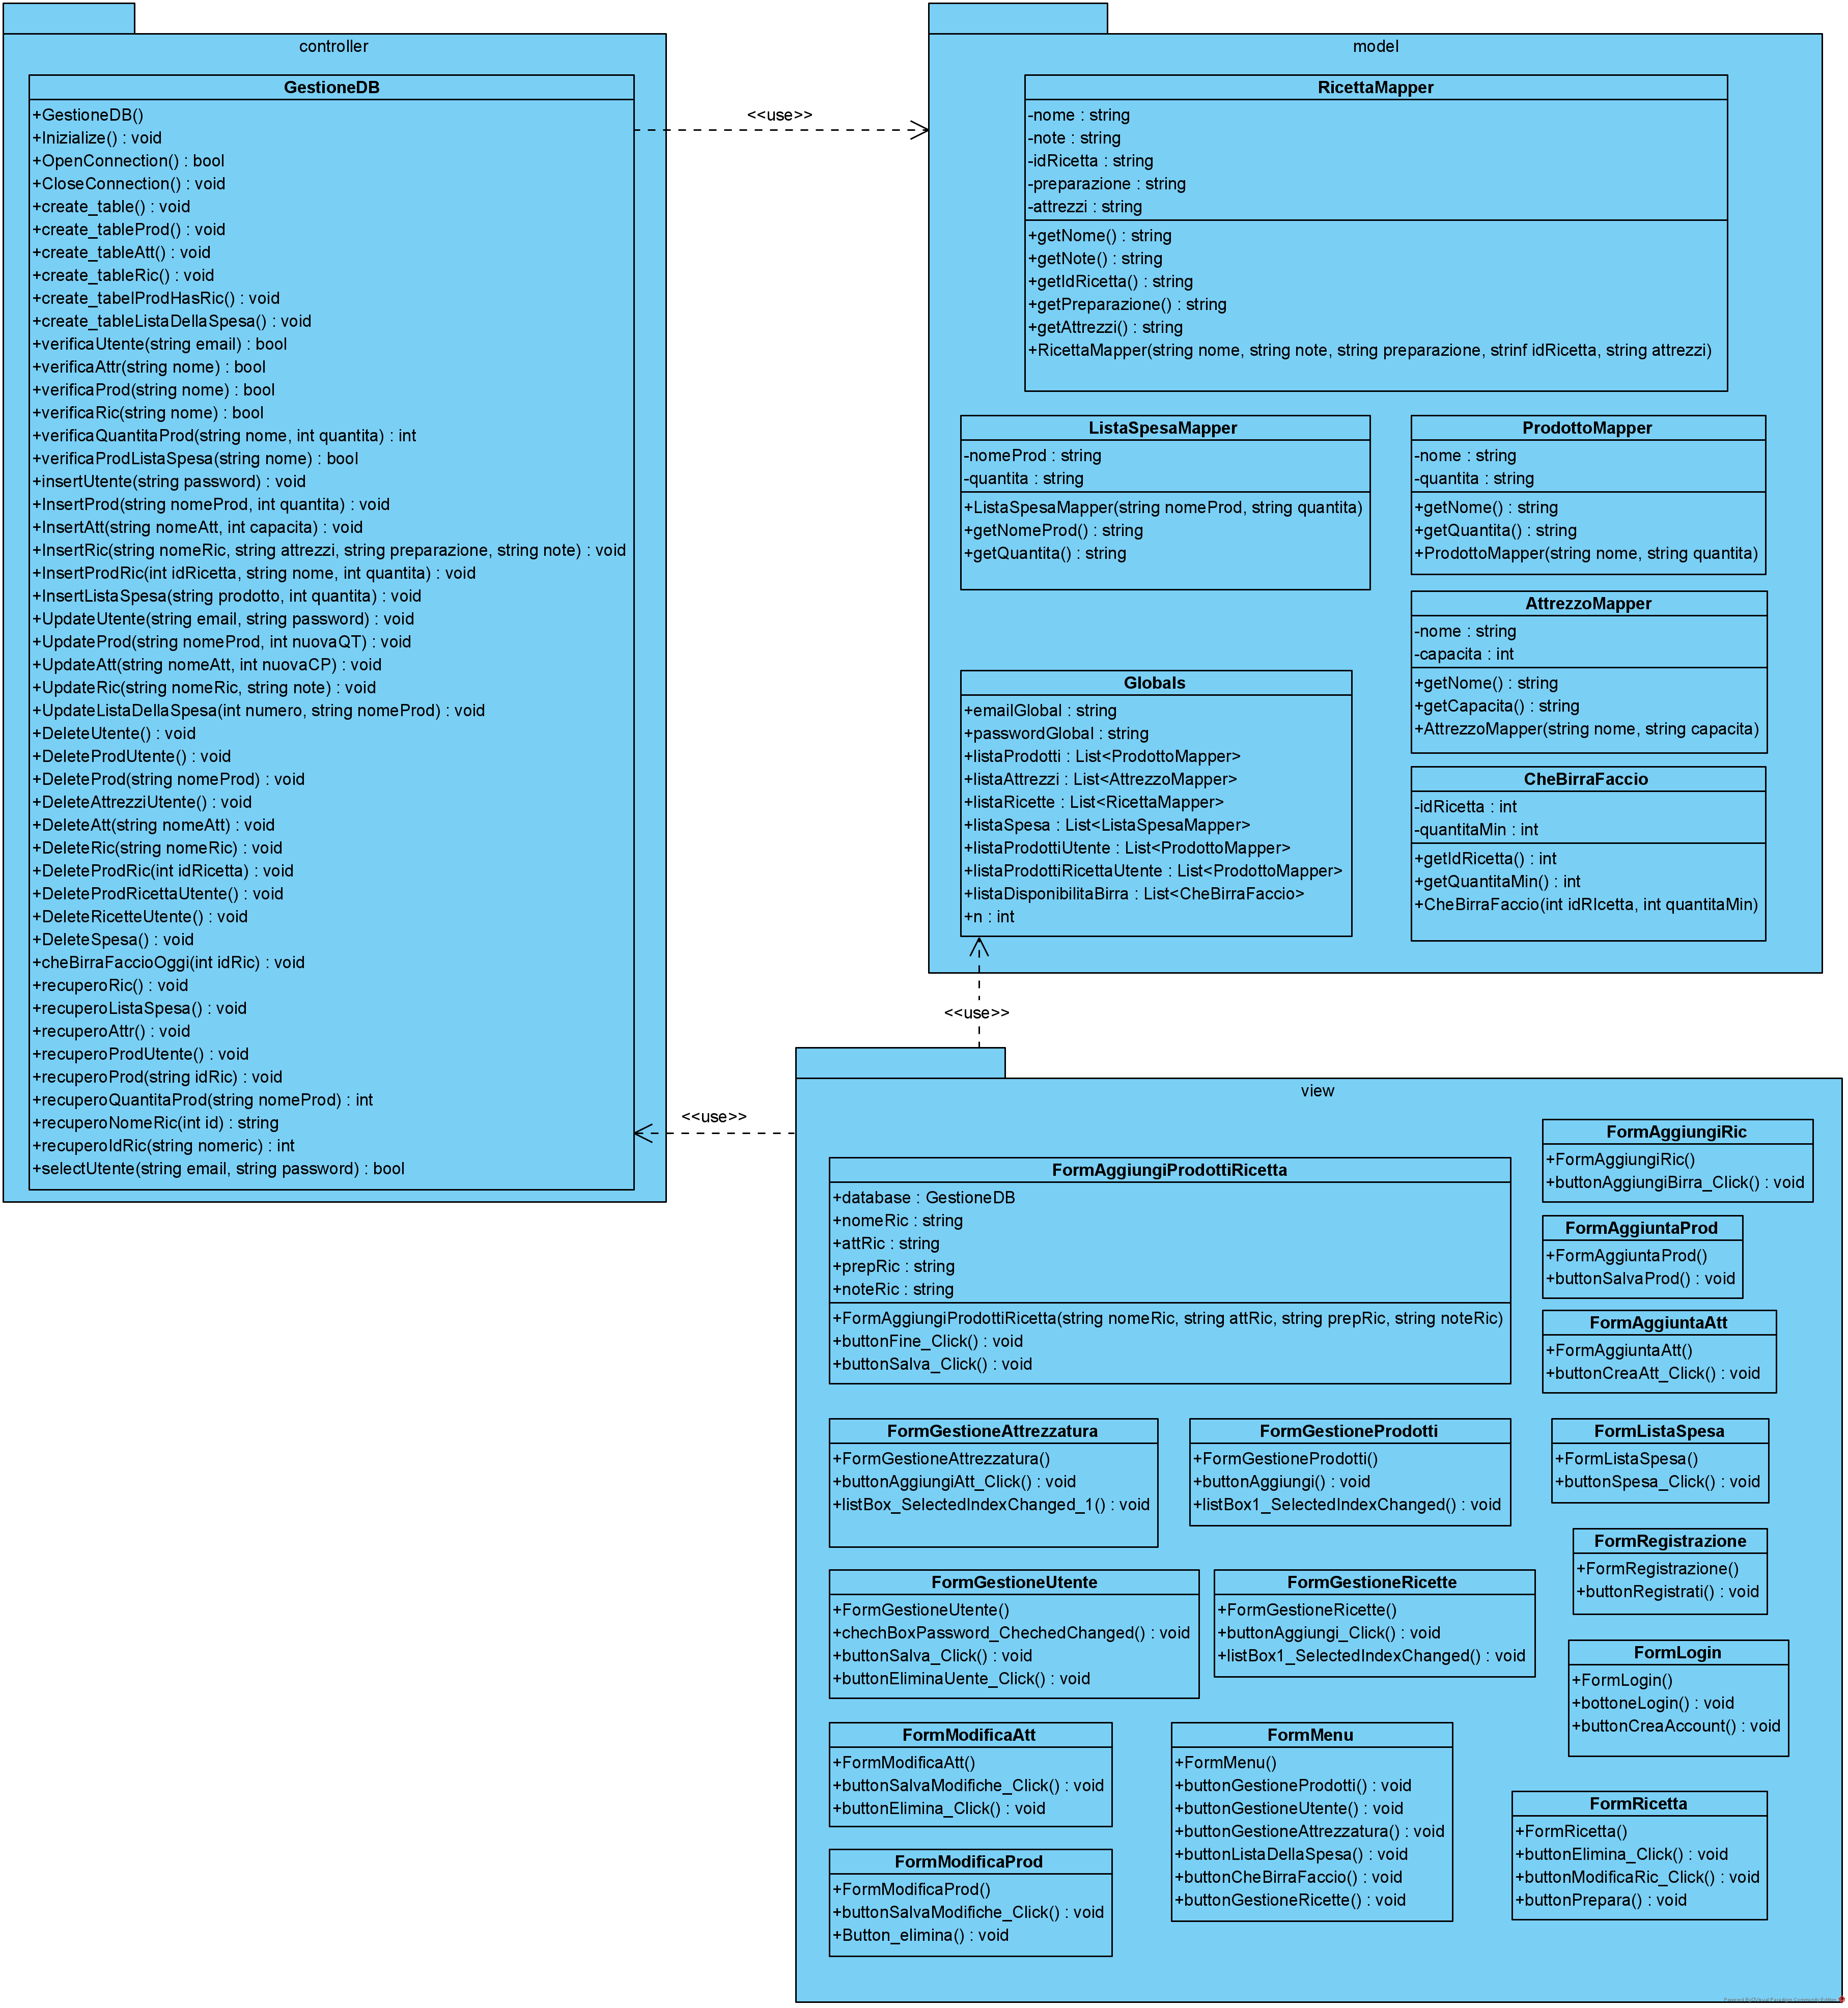
\includegraphics[scale=0.40]{Immagini/Design Model_Brew Day!_definitivo.png}
\subsection{Diagramma dell'architettura software}
In questo diagramma viene mostrata l'architettura dell'applicazione sviluppata.
L'architettura richiama il modello MVC:
\begin{itemize}
    \item Model: comprende le classi che strutturano l'applicazione;
    \item View: comprende tutte le classi che formano le finestre che costituiscono l'interfaccia per l'utente;
    \item Controller: è rappresentato dalla classe mediatrice tra View e il database esterno contenente i dati.
\end{itemize}
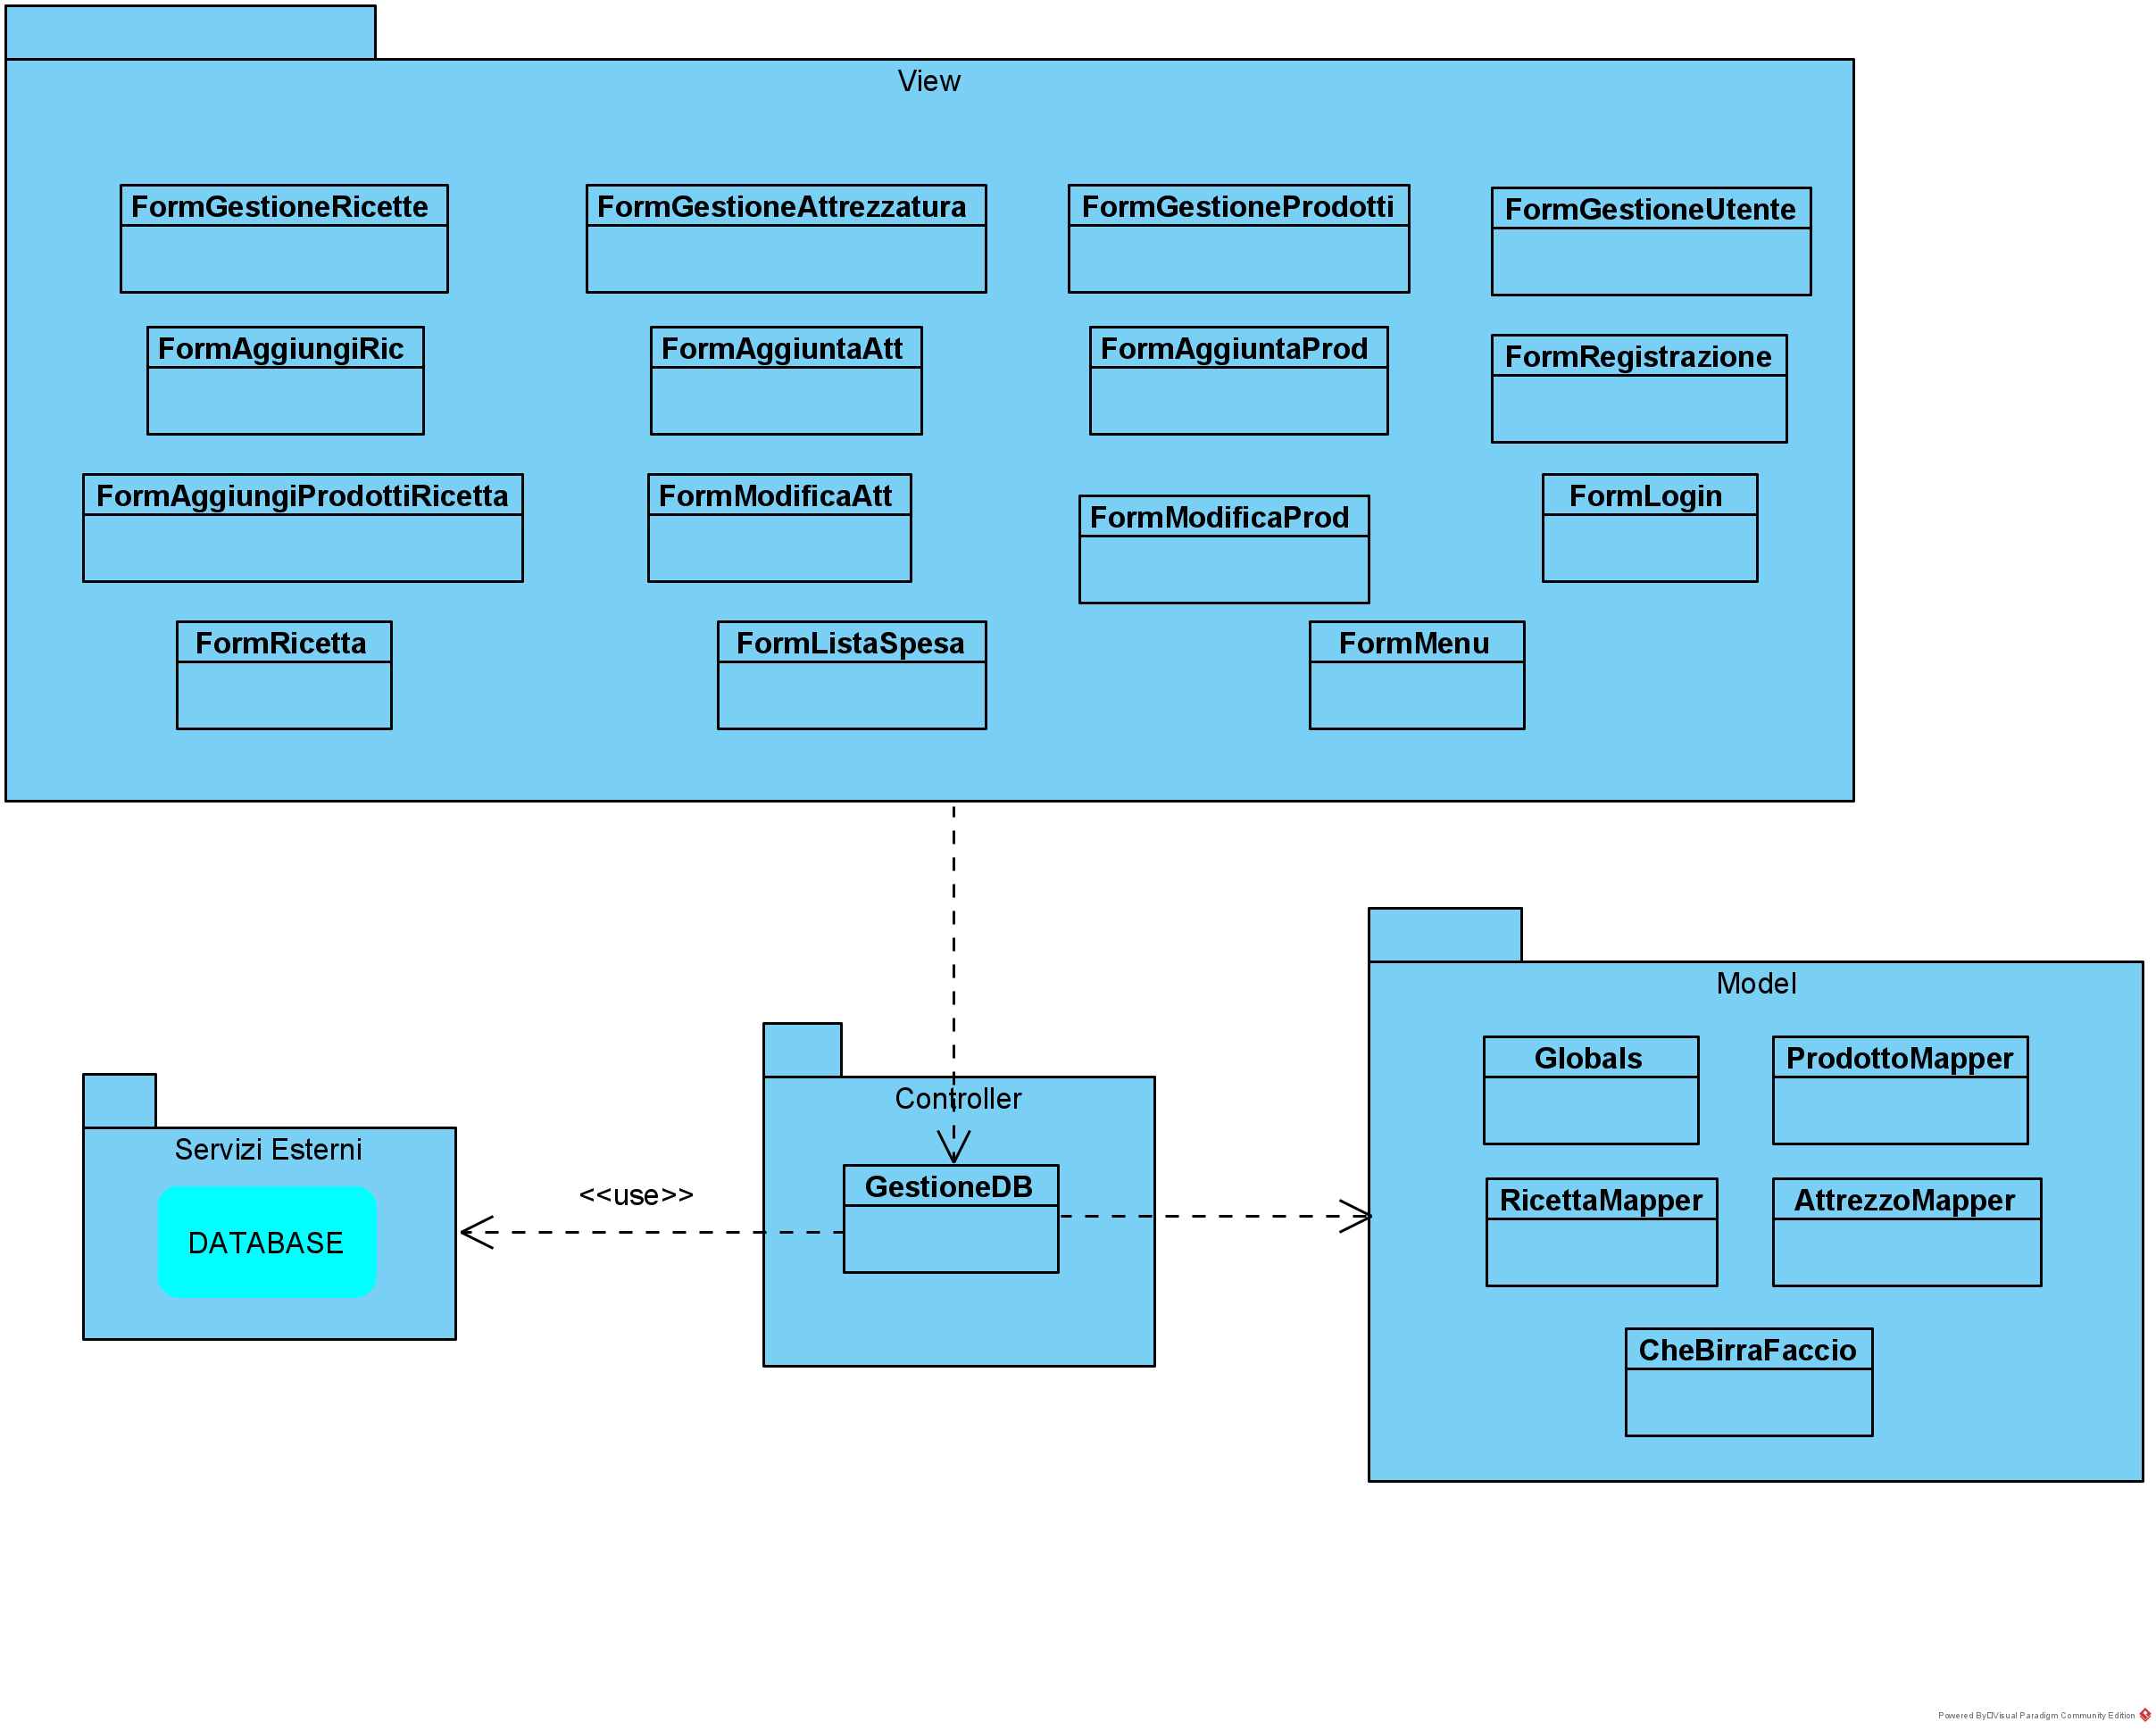
\includegraphics[scale=0.70]{Immagini/Diagramma Architettura Software_Brew Day!.png}

\newpage
\subsection{Diagramma di sequenza}
In questo diagramma viene mostrato l'intero funzionamento dell'applicazione.\\
Si parte dalla fase di registrazione in cui si inserisce email e password, queste credenziali vengono, dopo i dovuti controlli, salvati nel database. Questo passaggio permette di creare un account per salvare i prodotti, gli attrezzi e le ricette appartenenti all'utente.\\
Successivamente ci sarà la fase di login in cui, inserendo le proprie credenziali, si potrà accedere al menù principale dell'applicazione.\\
Dal menù è possibile svolgere diverse operazioni, manipolando diversi campi:
\begin{itemize}
    \item Profilo:
        \subitem - modificare il proprio profilo cambiando la password;
        \subitem - eliminare il proprio account.
    \item Prodotti:
        \subitem - aggiungere un nuovo prodotto con tutti i dati relativi ad esso (nome e quantità);
        \subitem - modificare la quantità di un prodotto esistente;
        \subitem - eliminare un prodotto esistente.
    \item Attrezzatura:
        \subitem - aggiungere un nuovo attrezzo con tutti i dati relativi ad esso (nome e capacità);
        \subitem - modificare la capacità di un attrezzo esistente
        \subitem - eliminare un attrezzo esistente.\\
        In questa applicazione l'attrezzatura è puramente a scopo illustrativo. Questa sezione tiene solamente traccia degli attrezzi che si possiedono, non viene considerata per la preparazione di una ricetta o nella funzionalità "Che Birra Faccio Oggi?".
    \item Ricette:
        \subitem - aggiungere una nuova ricetta con tutti i dati relativi ad essa (nome, elenco prodotti, elenco attrezzi, preparazione e note);
        \subitem - modificare le note di una ricetta esistente;
        \subitem - eliminare una ricetta esistente;
        \subitem - preparare una ricetta inserendo la quantità.\\
        La modifica di una ricetta riguarda solo le note, in quanto si crede che una volta inserita questa non vari nel tempo, mentre è utile poter modificare le note che riportano un'informazione personale riguardante la ricetta.
    \item "Che Birra Faccio Oggi?":
        \subitem è una funzionalità speciale che permette di ottenere un consiglio riguardo la ricetta da preparare. La ricetta ottenuta grazie a questa funzionalità è quella di cui si possono fare più litri con i prodotti presenti in quel momento nella propria dispensa.\\
        Questa funzionalità restituisce semplicemente un consiglio su quale birra produrre, mostrando nome e quantità massima supportata dai prodotti presenti in dispensa, poi sarà l'utente a scegliere quale ricetta e quanta prepararne.
    \item Lista della spesa:
        \subitem è una funzionalità che permette di vedere quali prodotti mancano nella dispensa per poter preparare le varie ricette, una volta selezionata questa voce si visualizzerà la lista e si avrà la possibilità di cancellarla una volta comprato i prodotti.\\
        La lista della spesa viene solo visualizzata in modo che poi sia l'utente a scegliere cosa comprare e potrà in autonomia cancellare la lista ed aggiornate i prodotti.
\end{itemize}
\newpage
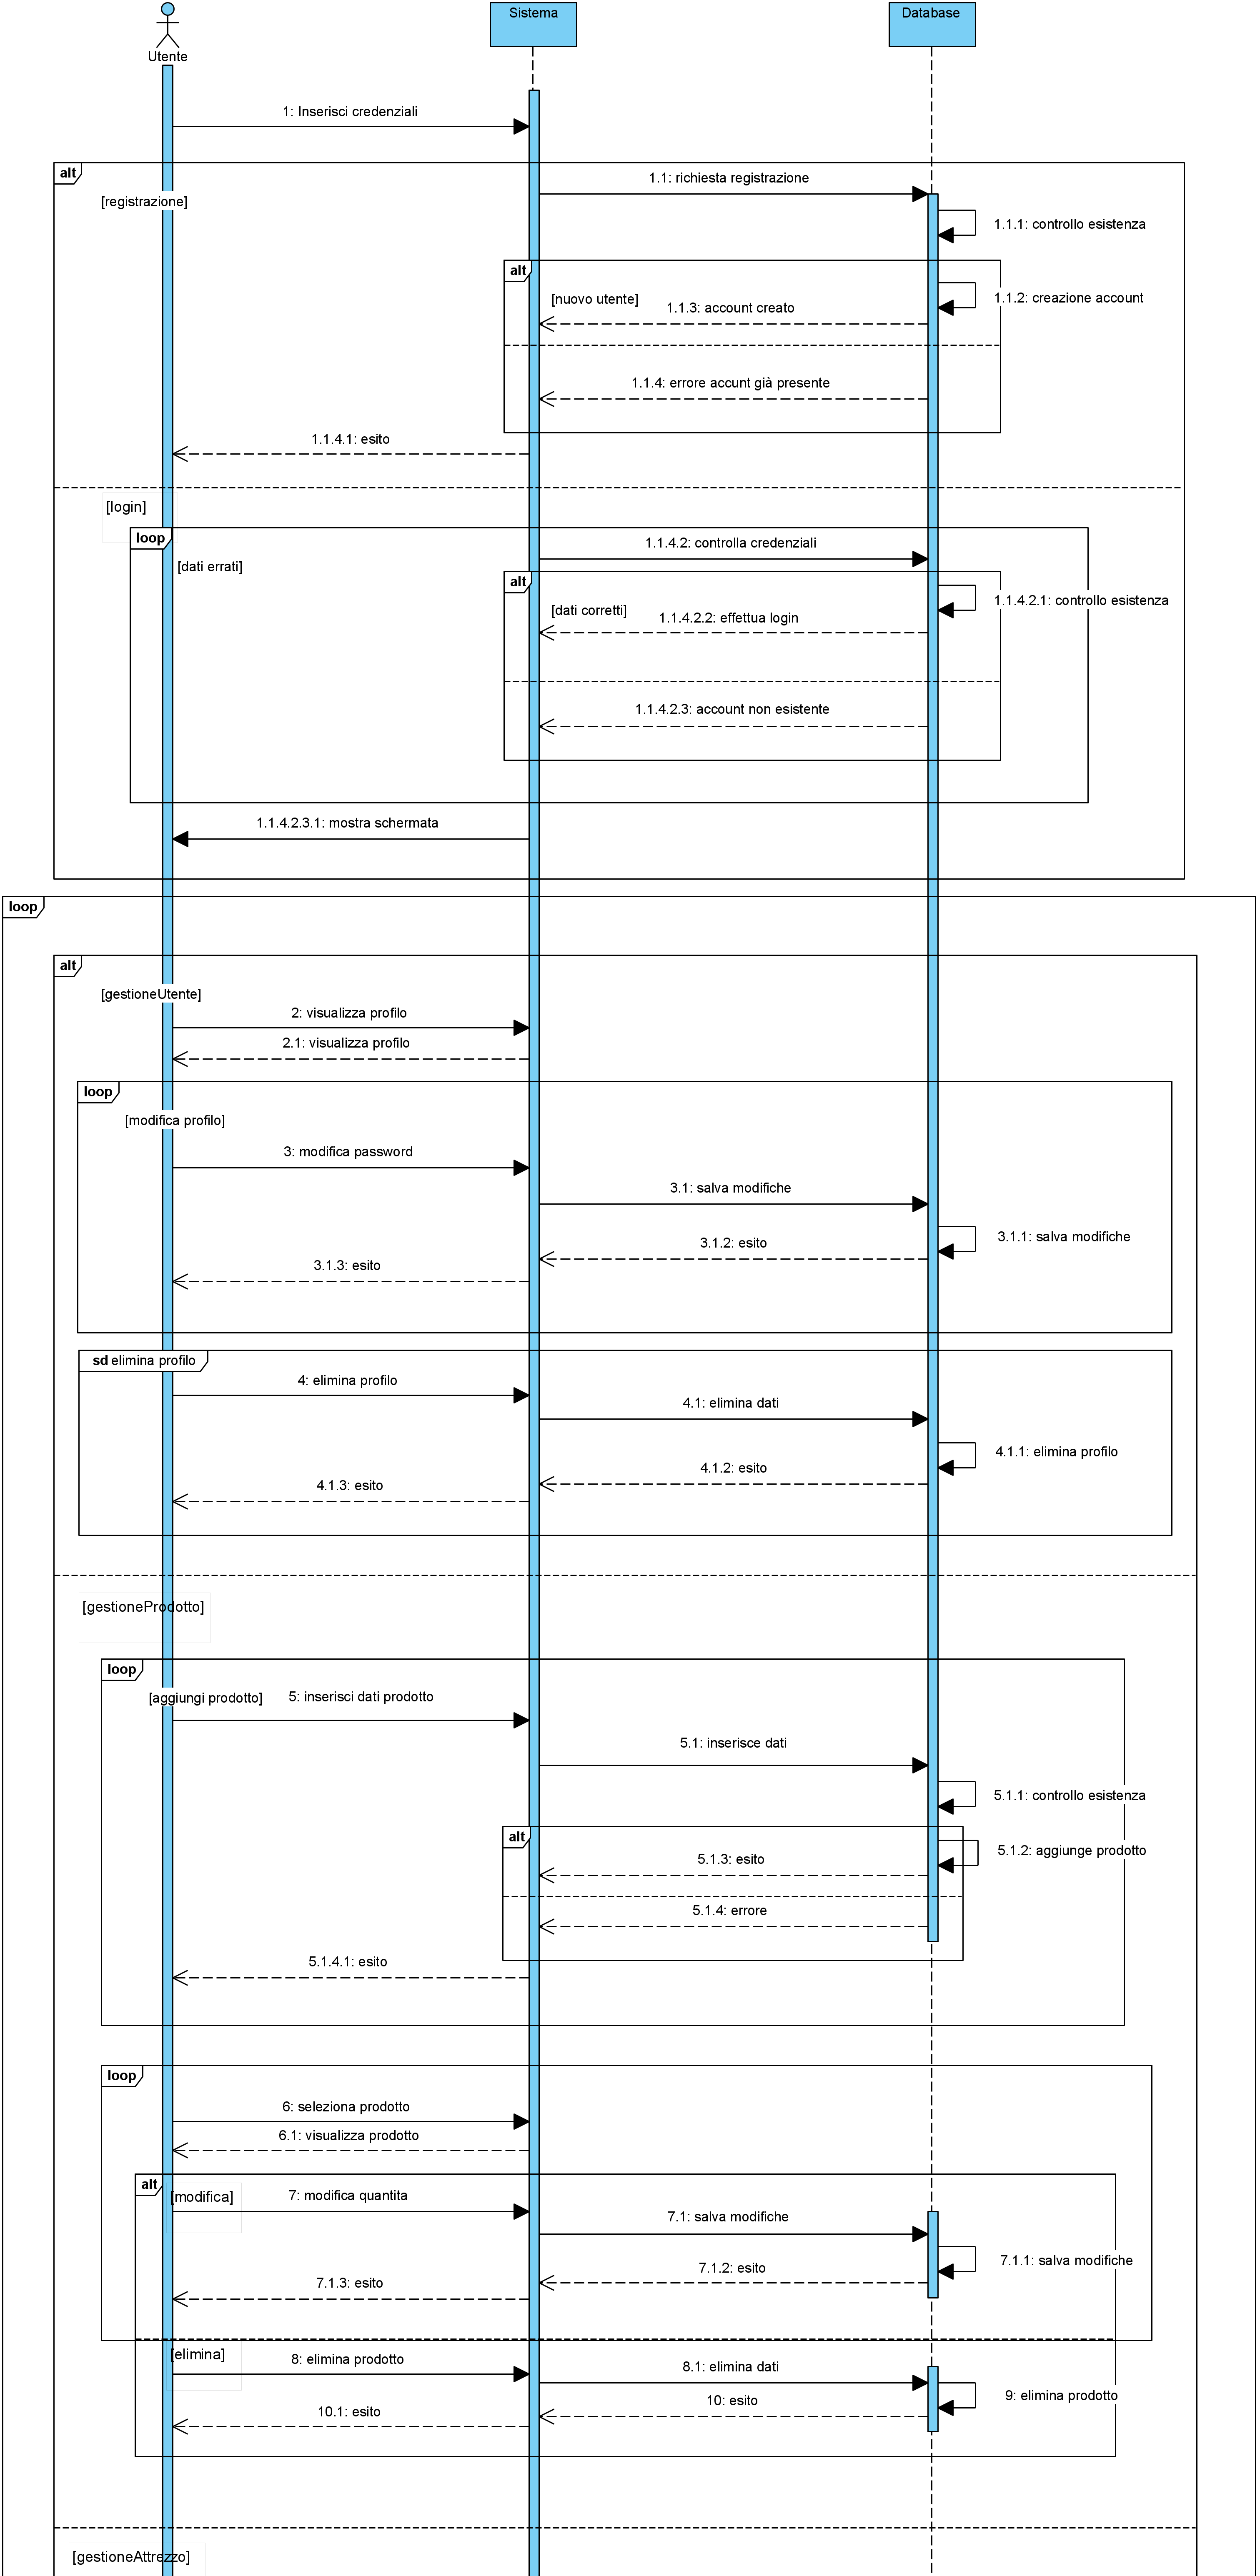
\includegraphics[scale=0.40]{Immagini/Sequence Diagram_Brew Day!_definitivo_1.png}
\newpage
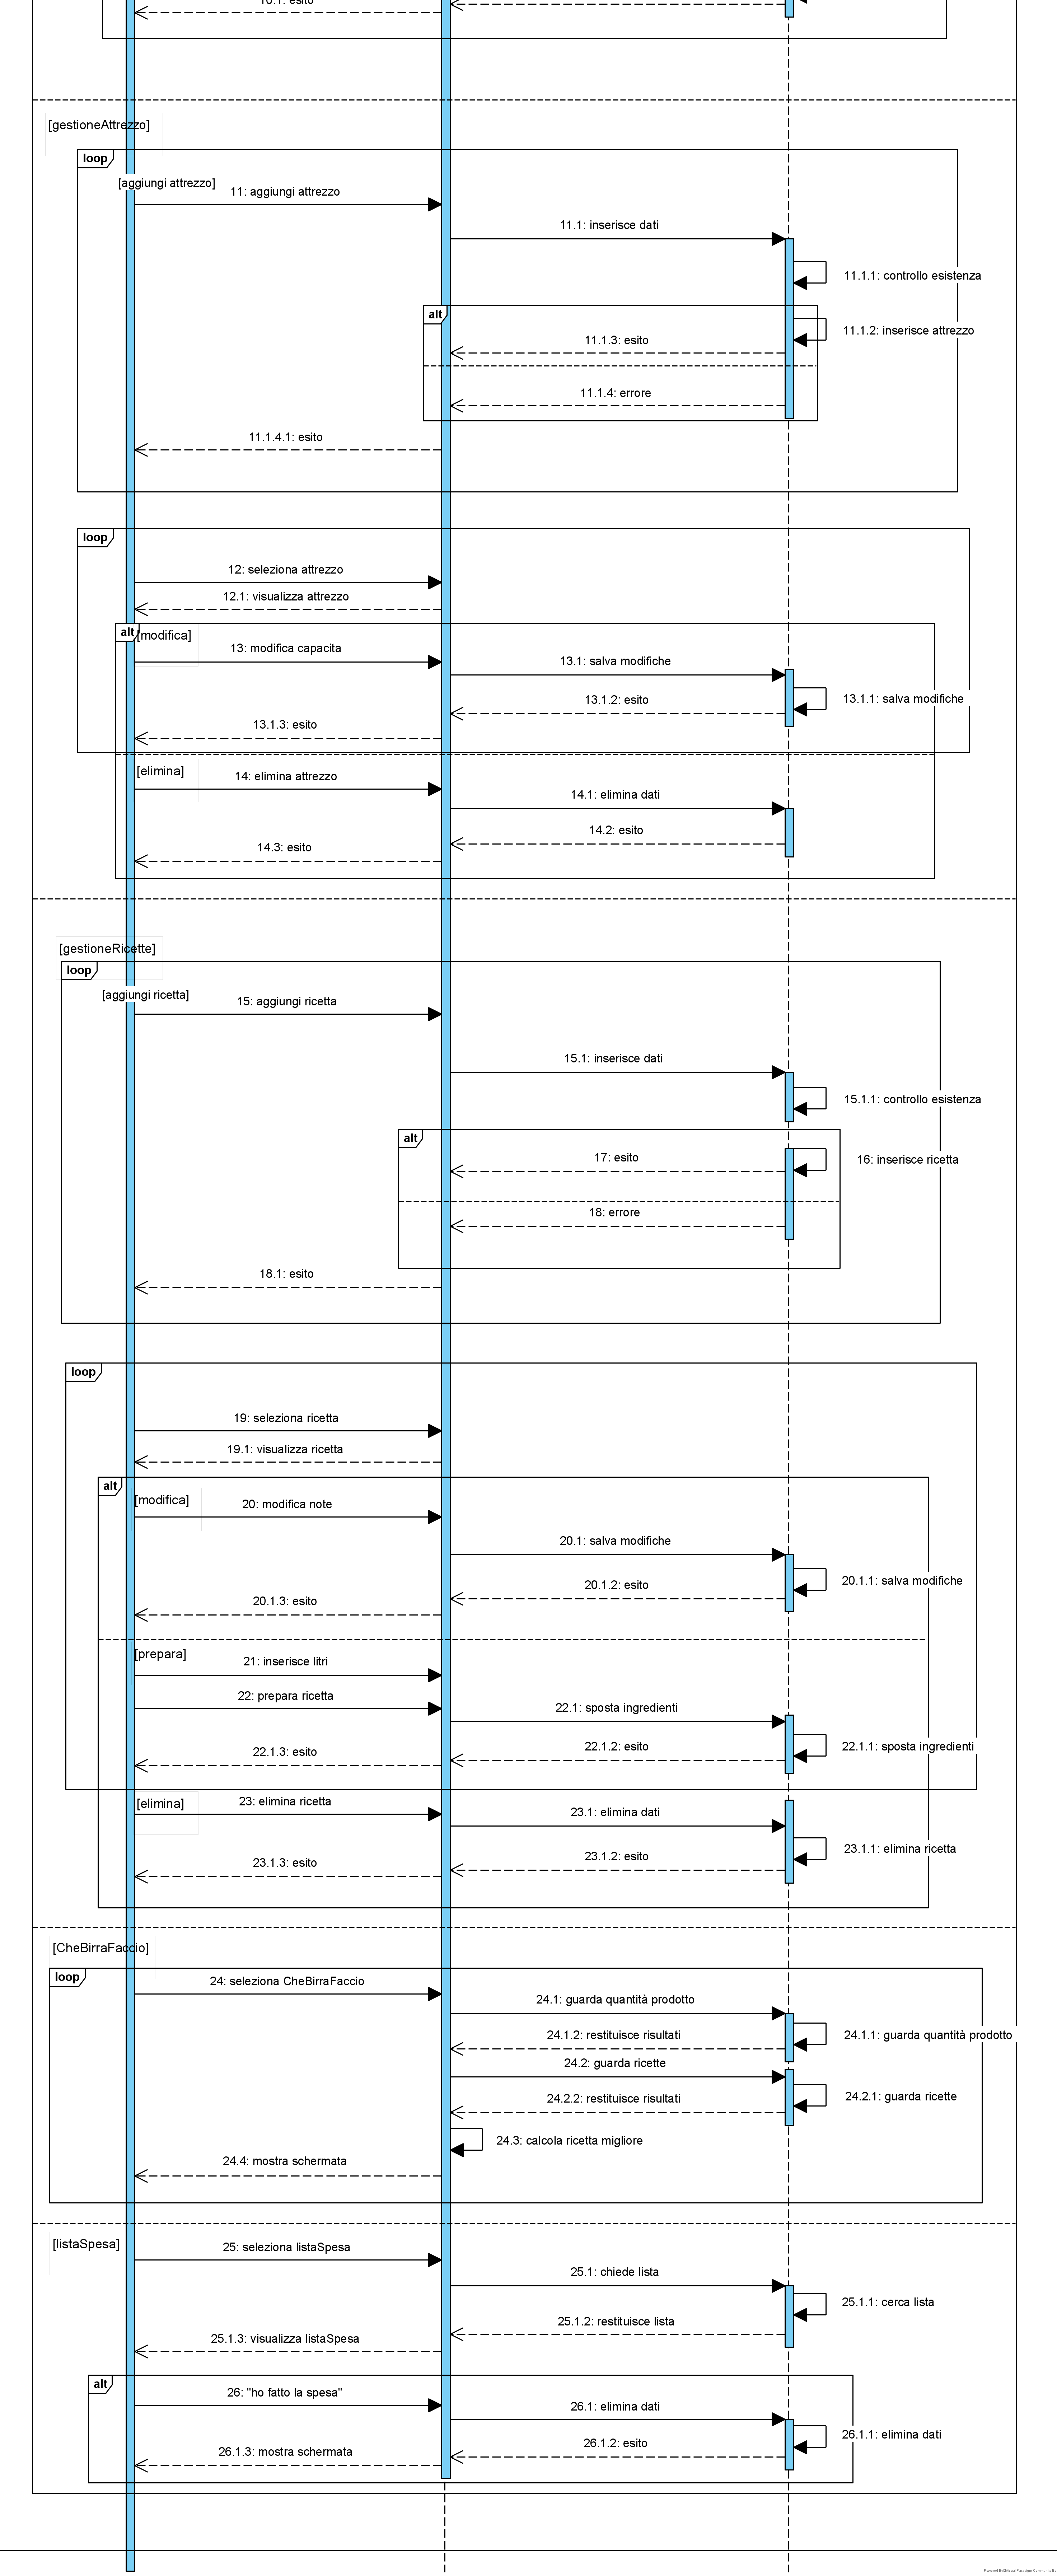
\includegraphics[scale=0.40]{Immagini/Sequence Diagram_Brew Day!_definitivo_2.png}

\newpage

\subsection{Diagramma di sequenza di progettazione}
Questo diagramma mostra in modo più specifico il funzionamento del caso d'uso gestioneRicette.\\\\\
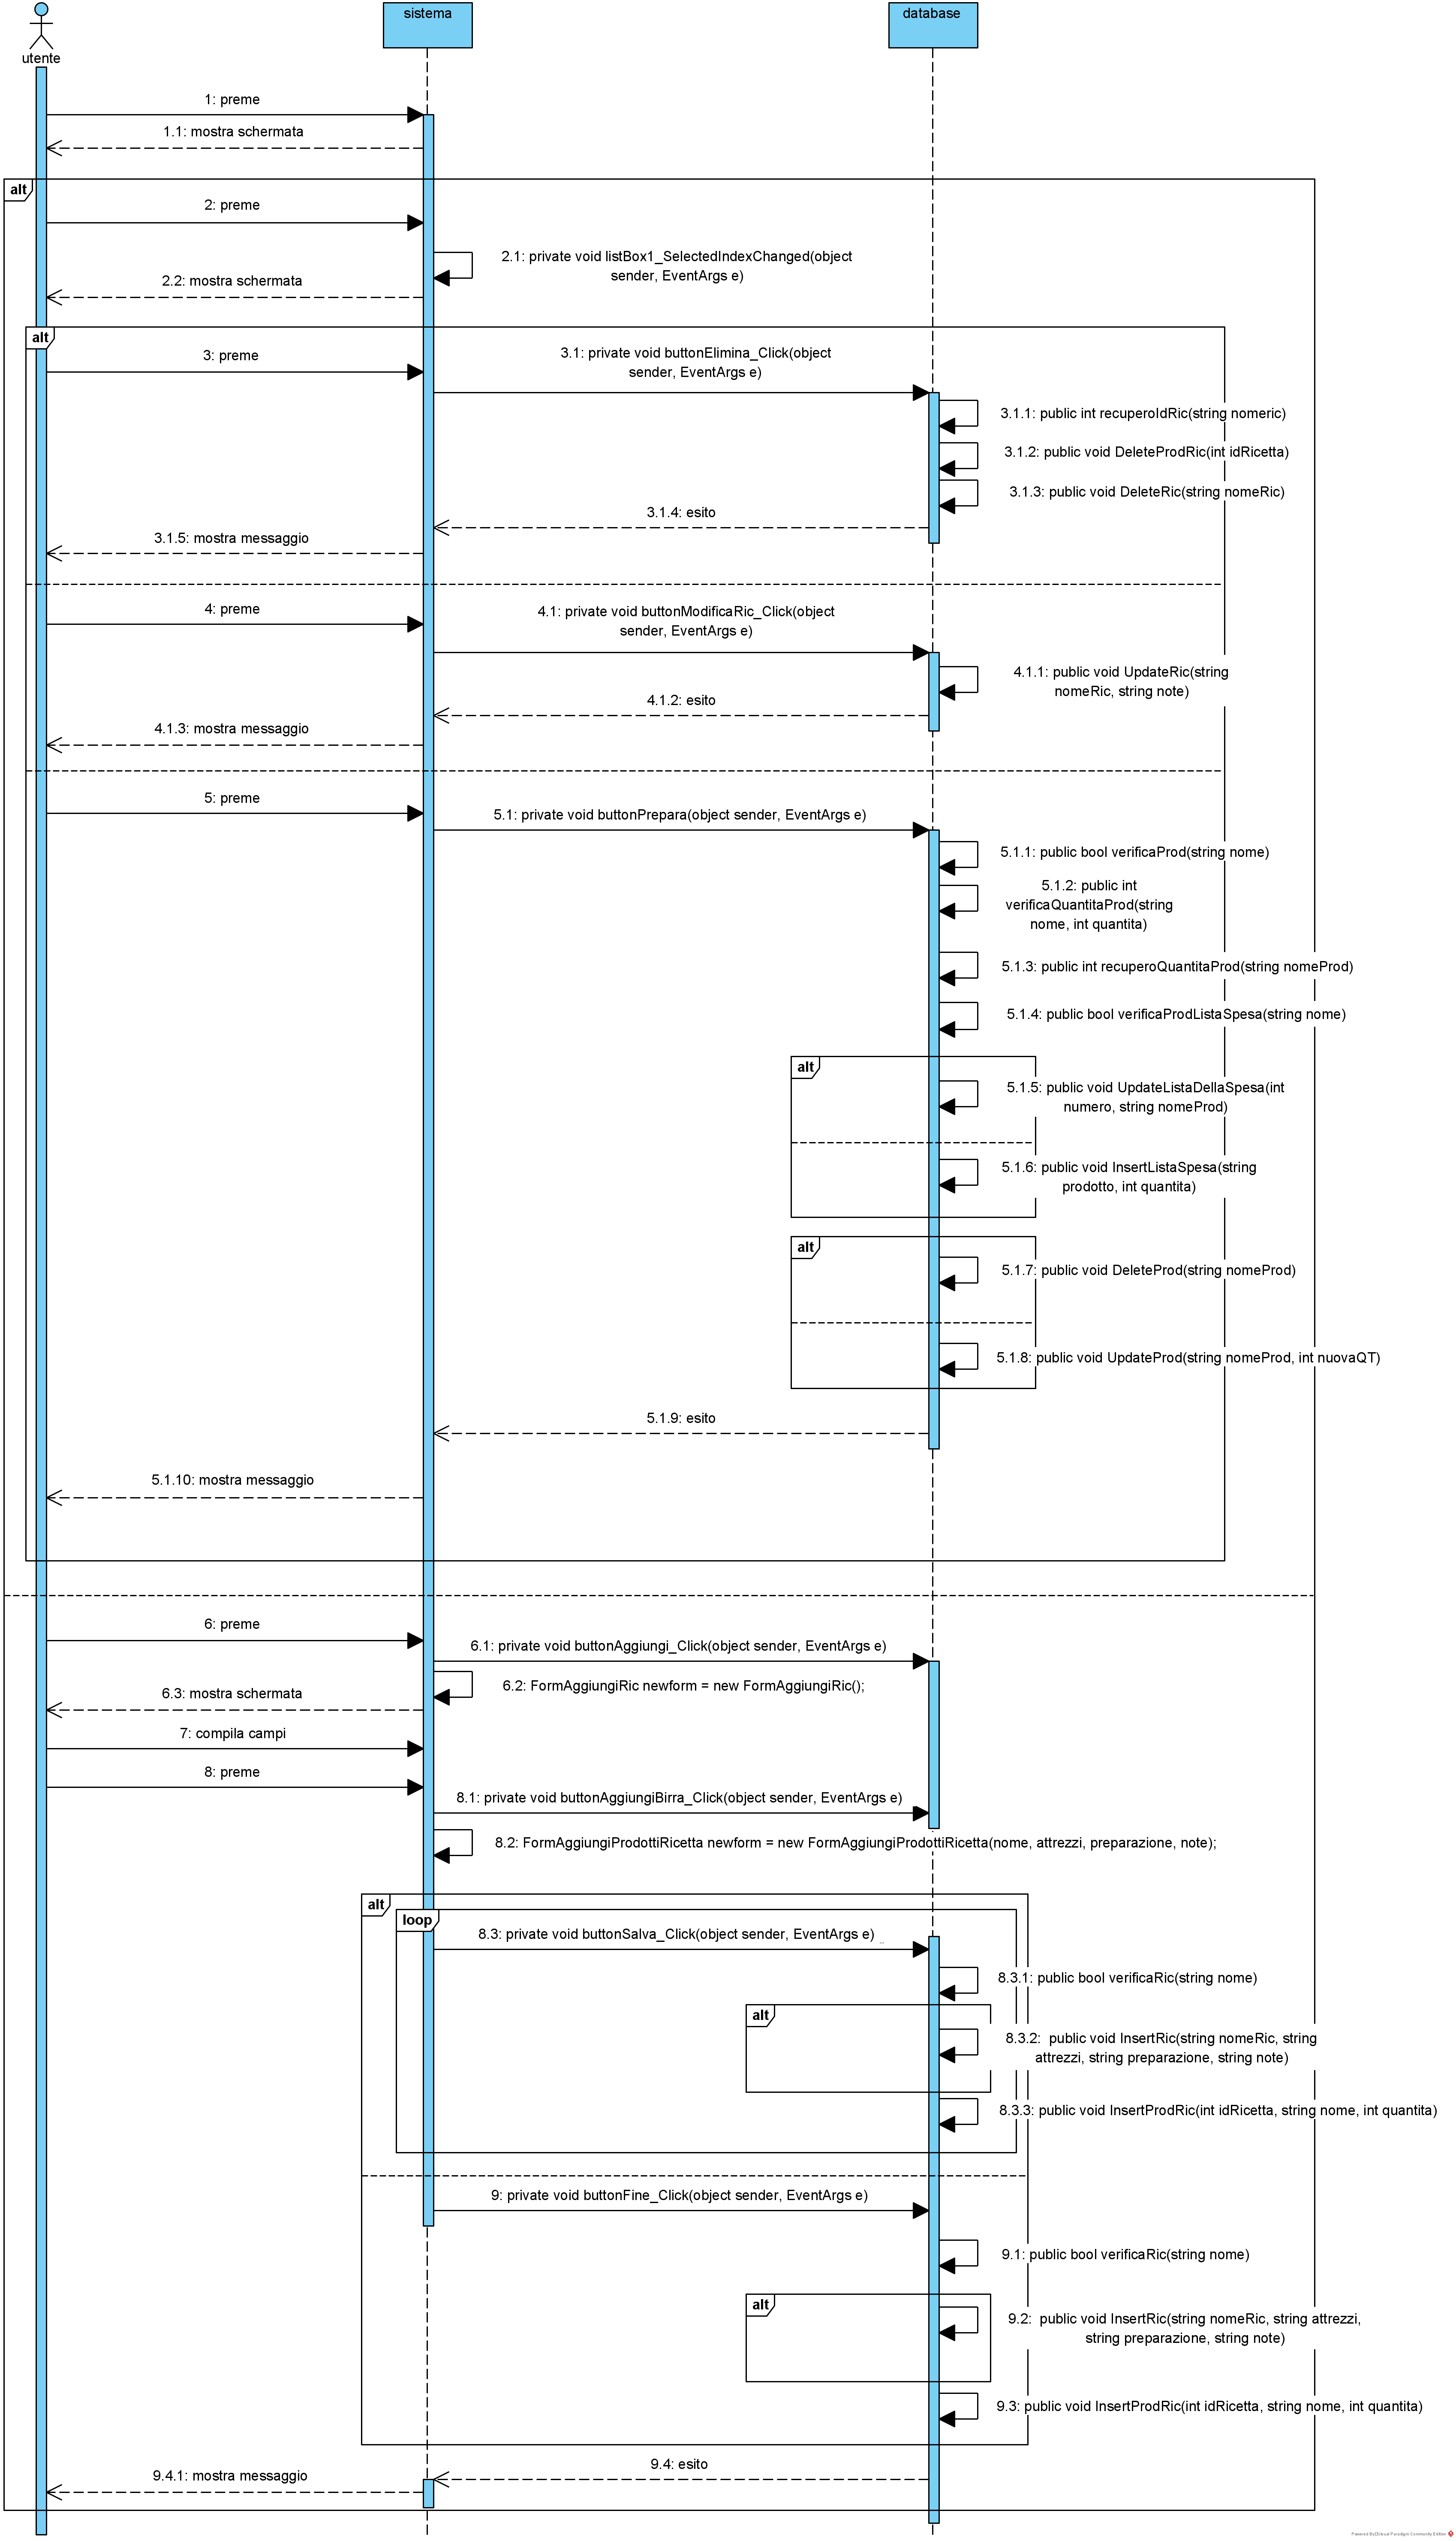
\includegraphics[scale=0.43]{Immagini/Sequence Diagram gestioneRicette.png}
\subsection{Diagramma di stato}
Questo diagramma a stati mostra la funzionalità login.\\\\

\includegraphics[scale=0.60]{Immagini/State Machine Diagram Login_Brew Day!.png}
\subsection{Diagramma di attività}
Questo diagramma mostra mostra la funzionalità registrazione.\\\\
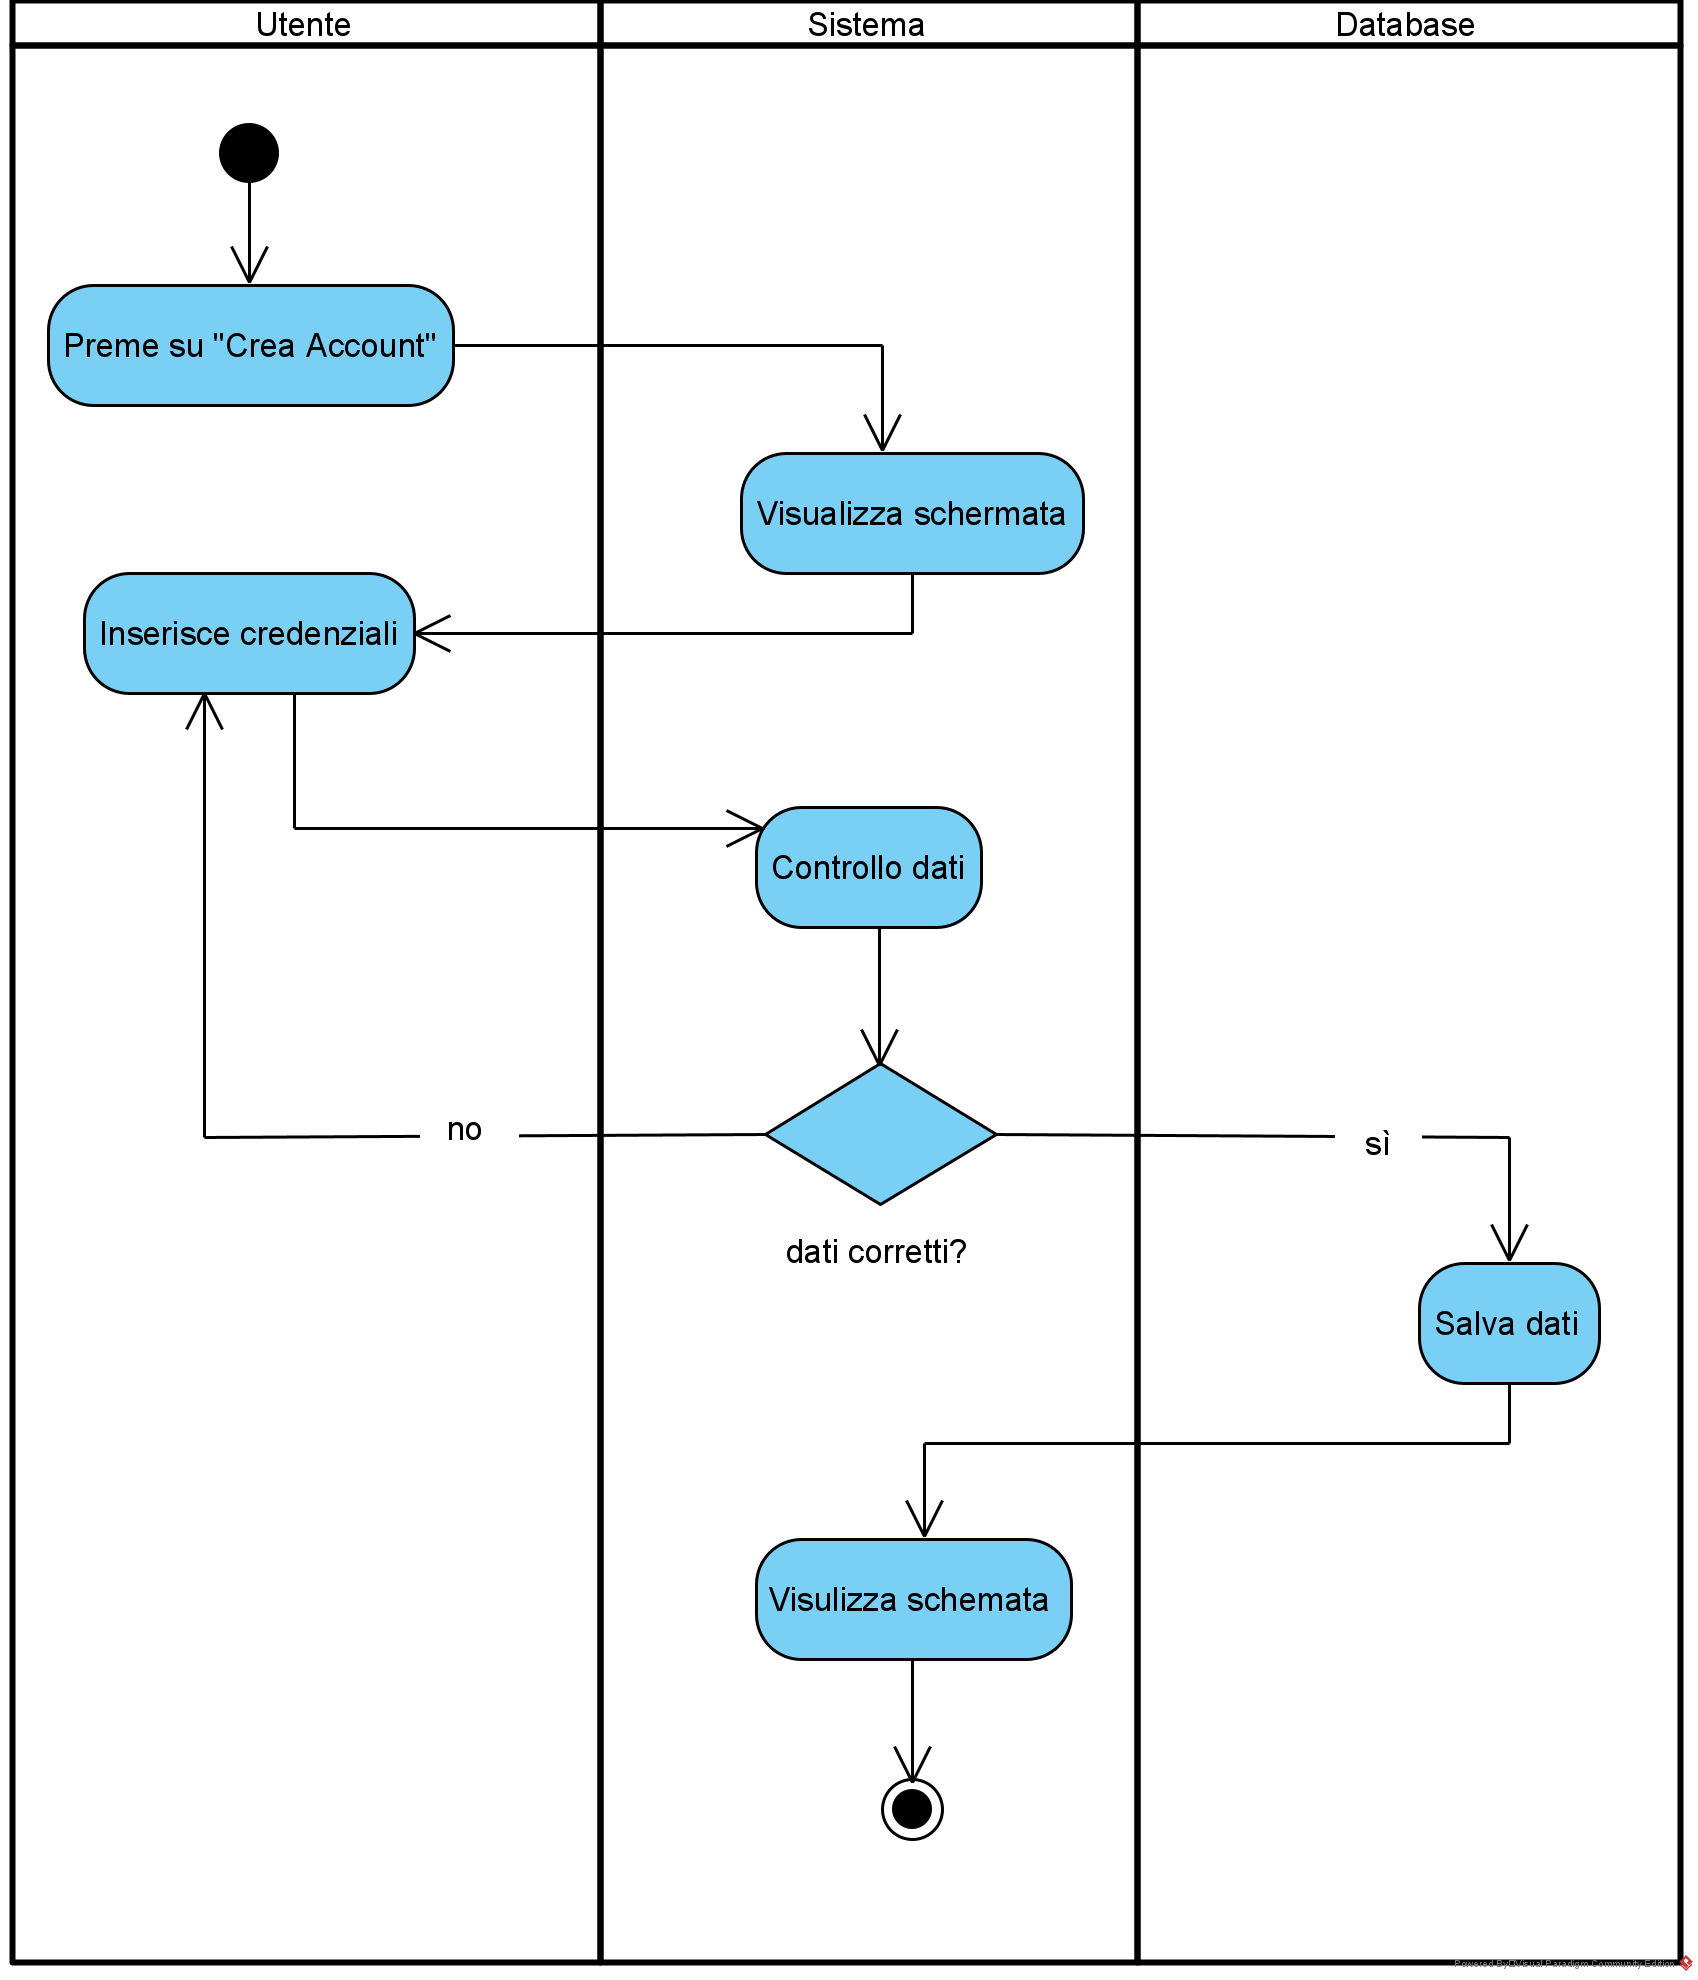
\includegraphics[scale=0.50]{Immagini/Activity Diagram Registrazione_Brew Day!.png}
\subsection{Diagramma EER}
Questo diagramma rappresenta la struttura del database creato come appoggio all'applicazione.\\\\
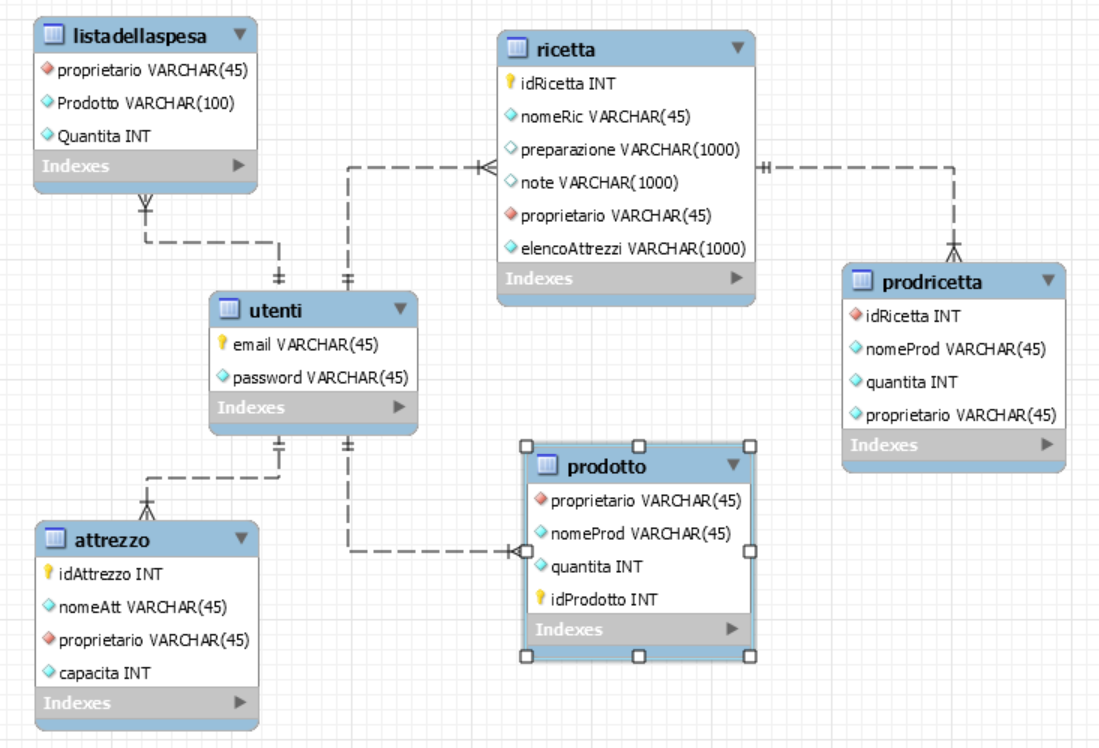
\includegraphics[scale=0.50]{Immagini/diagrammaER.PNG}
\\E' stato utilizzato un database esterno di supporto dell'applicazione in quanto è possibile installarla su dispositivi diversi e recuperare le proprie informazioni.
\newpage

\section{Pattern}
\vphantom{}
\subsection{Singleton}
Questo pattern viene utilizzato dalla classe 'GestioneDB'. Questa classe ha il compito di svolgere tutte le operazioni che si interfacciano al database di supporto. Abbiamo introdotto questo pattern al fine di evitare errori di comunicazione, infatti è presente una sola classe mediatrice tra il database e le altre classi.\\\\
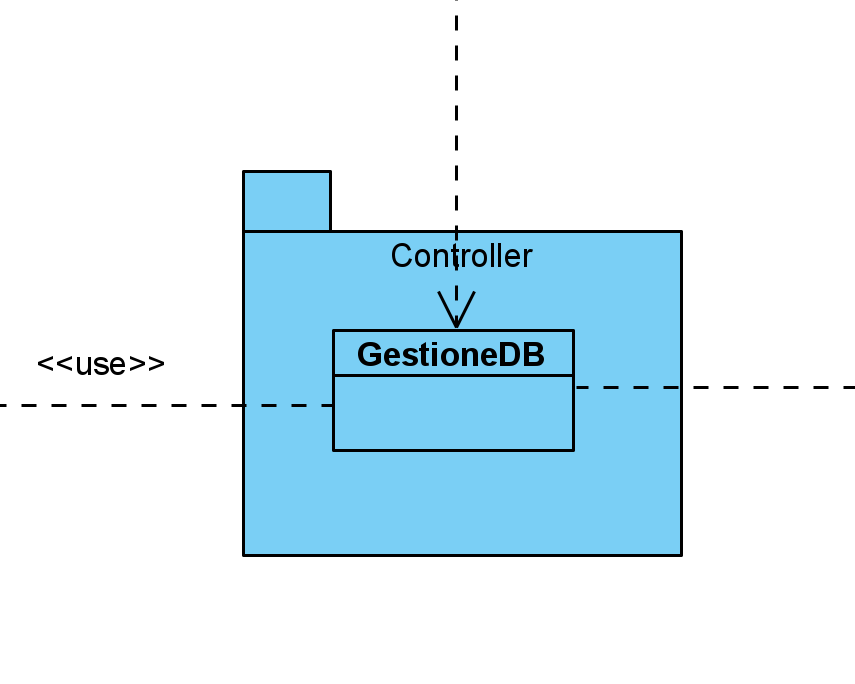
\includegraphics[scale=0.80]{Immagini/Singleton.png}
\subsection{Data Mapper}
Questo pattern viene utilizzato nella creazione delle classi che rappresentano gli oggetti manipolati nel database.
E' stato rivisitato il suo utilizzo rendendolo più semplice togliendo uno step intermedio.
Nel nostro caso vengono creati degli oggetti di tipo prodotto, ricetta e listaSpesa in modo da non dover richiedere ogni volta l'intervento del database.\\\\
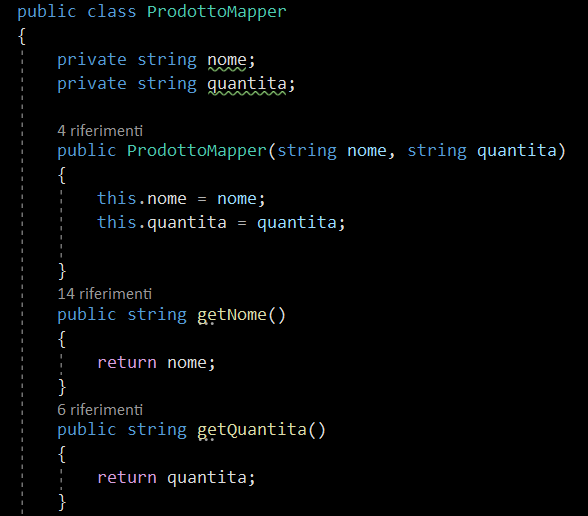
\includegraphics[scale=0.70]{Immagini/DataMapper.PNG}
\newpage
\subsection{Identity Field}
Questo pattern è presente in tutte le tabelle del database, ma viene utilizzato in modo particolare nelle funzionalità inerenti alla tabella Ricetta.
La chiave primaria idRicetta viene utilizzata per richiamare i prodotti contenuti nella tabella 'prodricetta' per le funzionalità di preparazione di una ricetta e "Che birra faccio oggi?".\\\\
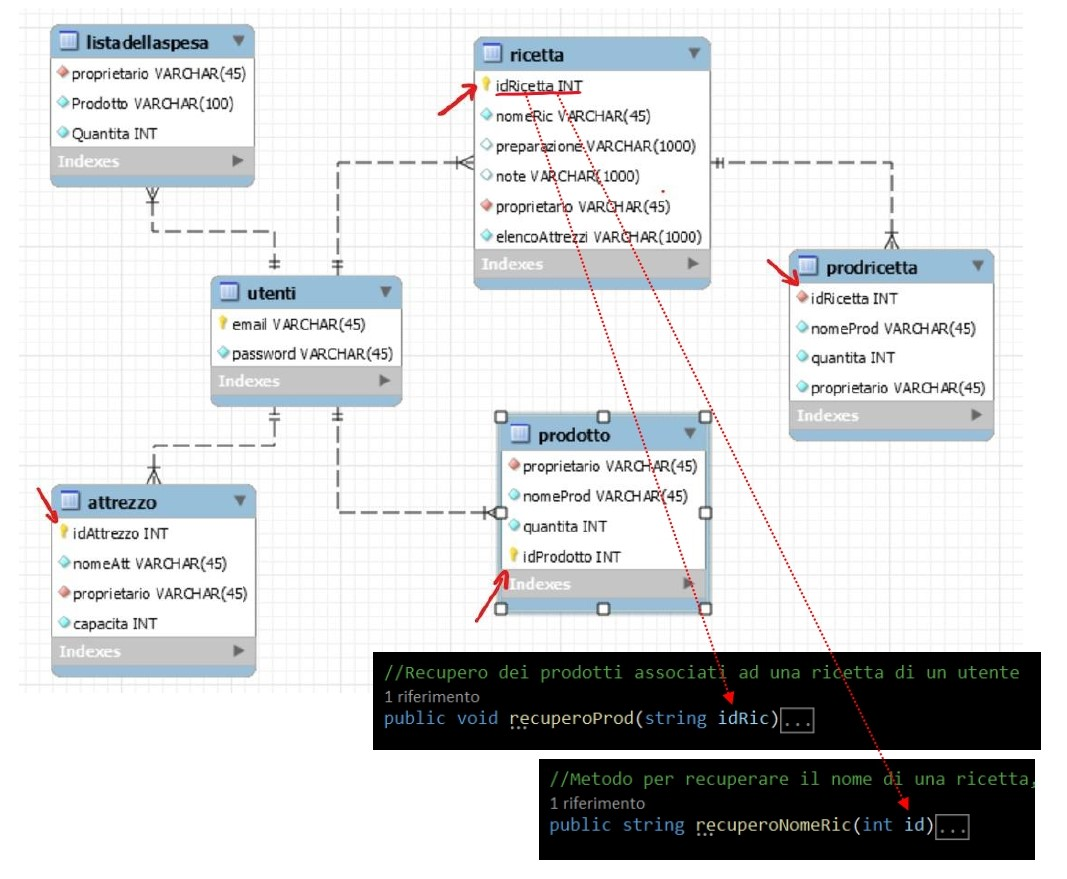
\includegraphics[scale=0.40]{Immagini/IdentityField.jpg}
\subsection{Association Table Mapping}
Questo pattern viene utilizzato nella tabella 'prodricetta' come collegamento tra le tabelle 'ricetta' e 'prodotto'. All'interno del database non è presente come un'associazione molti-a-molti, viene però utilizzata in questo modo nell'implementazione.\\\\ 
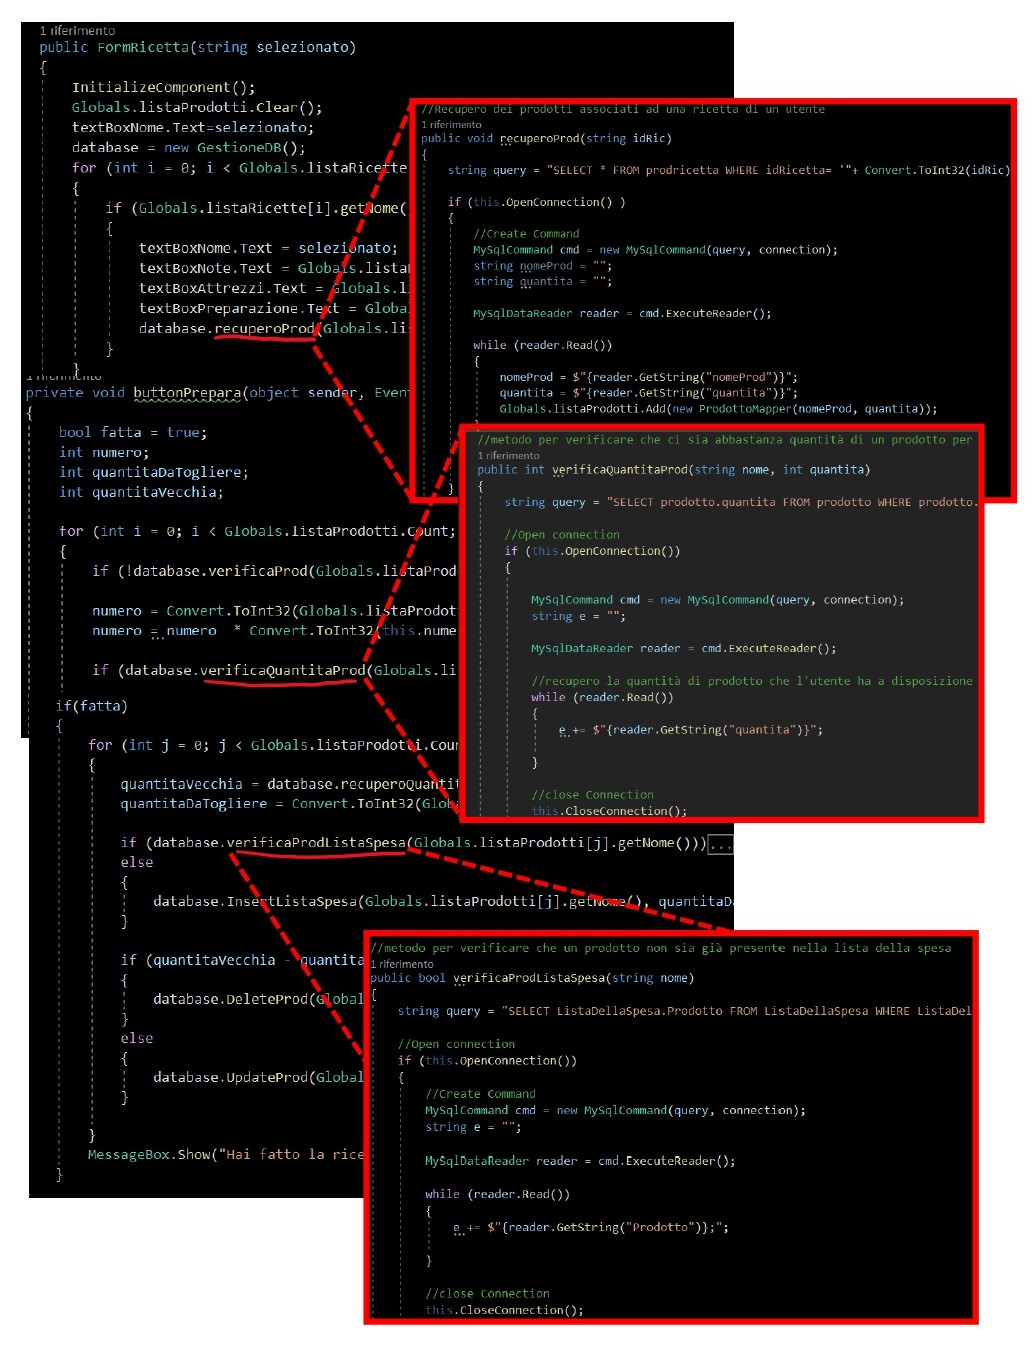
\includegraphics[scale=0.40]{Immagini/AssociationTableMapping_.jpg}
\subsection{Facade}
Questo pattern è presente nella gestione delle finestre, l'utente preme il bottone e il metodo che svolge questa funzionalità è semplice e nasconde la complessità dell'utilizzo dell'applicazione.
\newpage

\section{Analisi Understand}
Tramite l'utilizzo del software Understand è stata svolta un'analisi del codice e della struttura dell'applicazione sviluppata.\\\\
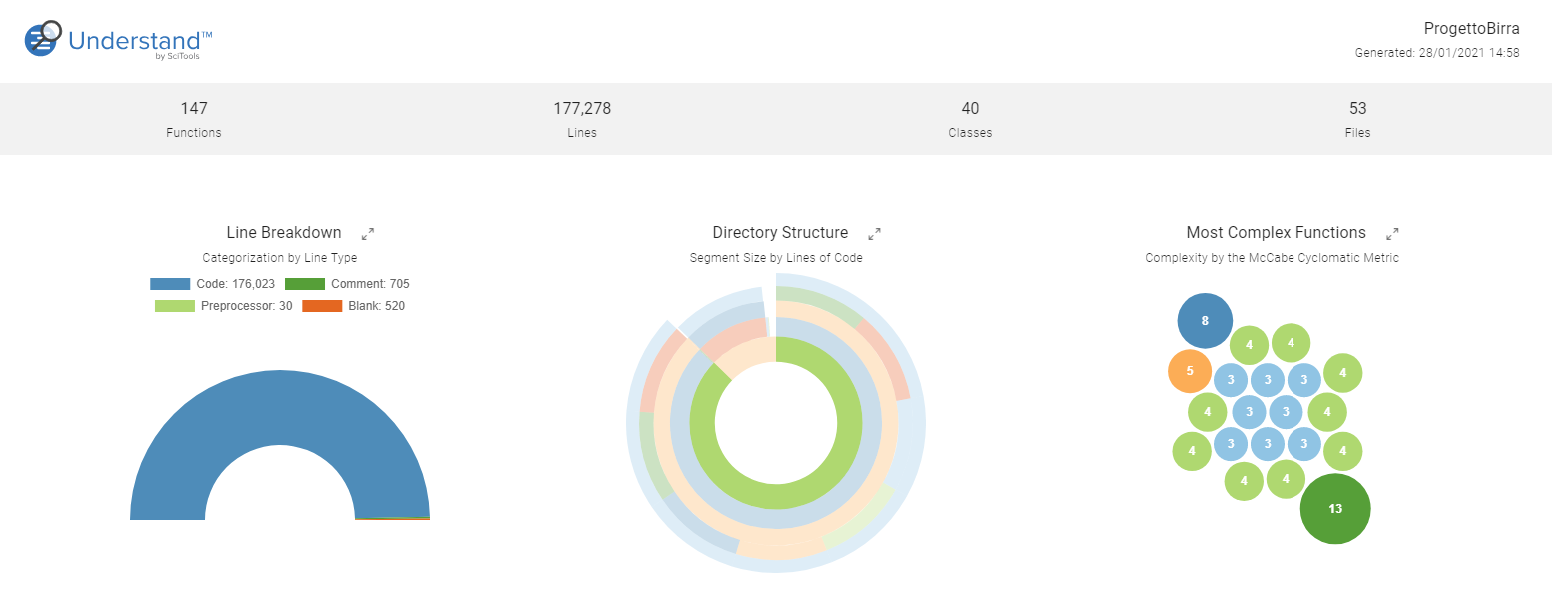
\includegraphics[scale=0.40]{Immagini/Understand_1.png}\\
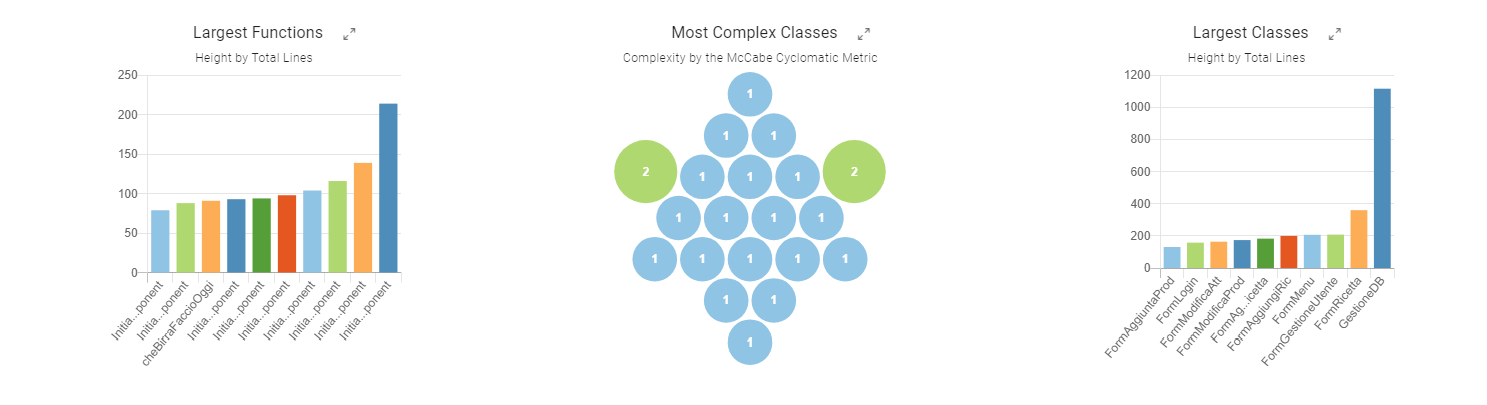
\includegraphics[scale=0.40]{Immagini/Understand_3.png}\\
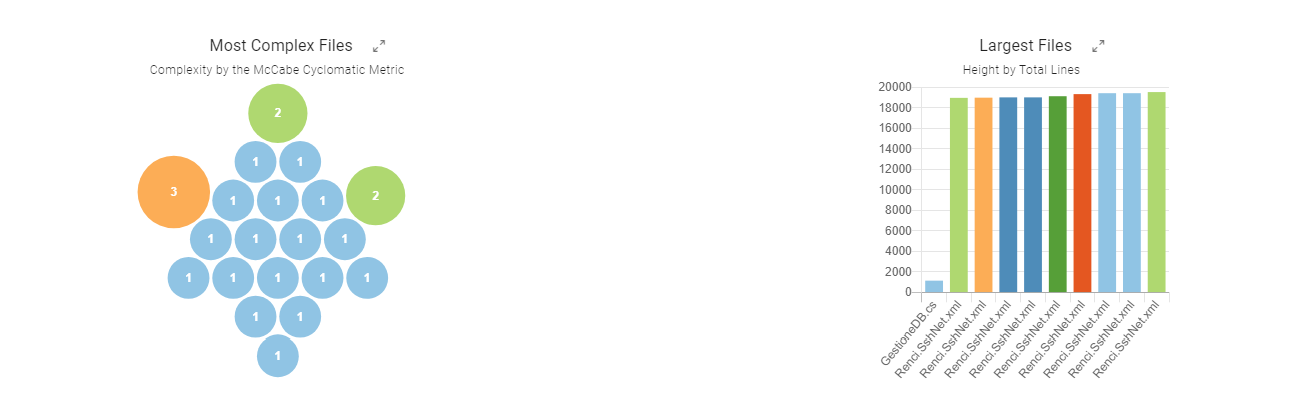
\includegraphics[scale=0.40]{Immagini/Understand_2.png}\\
\\Sono stati individuati alcuni antipatterns.
\subsection{God Class}
E' stata individuata la classe 'GestioneDB' come la classe che "sa tutto". Essa infatti contiene tutte le informazioni riguardanti tutte le funzioni svolte dall'applicazione.
\subsection{Accumulate and fire}
All'interno del progetto vengono usate variabili globali per facilitare la comunicazione tra le classi.
\subsection{Copy and paste programming}
All'interno del progetto sono presenti diversi metodi che svolgono la stessa funzione ma che è stato necessario implementare più volte perché comunicando con il database variava la tabella interessata;
\subsection{Reinventing the wheet}
E' stato usato un metodo già testato per effettuare la connessione con il database.

\section{Analisi Sonarqube}
Viene riportata la schermata di analisi del progetto software.\\\\
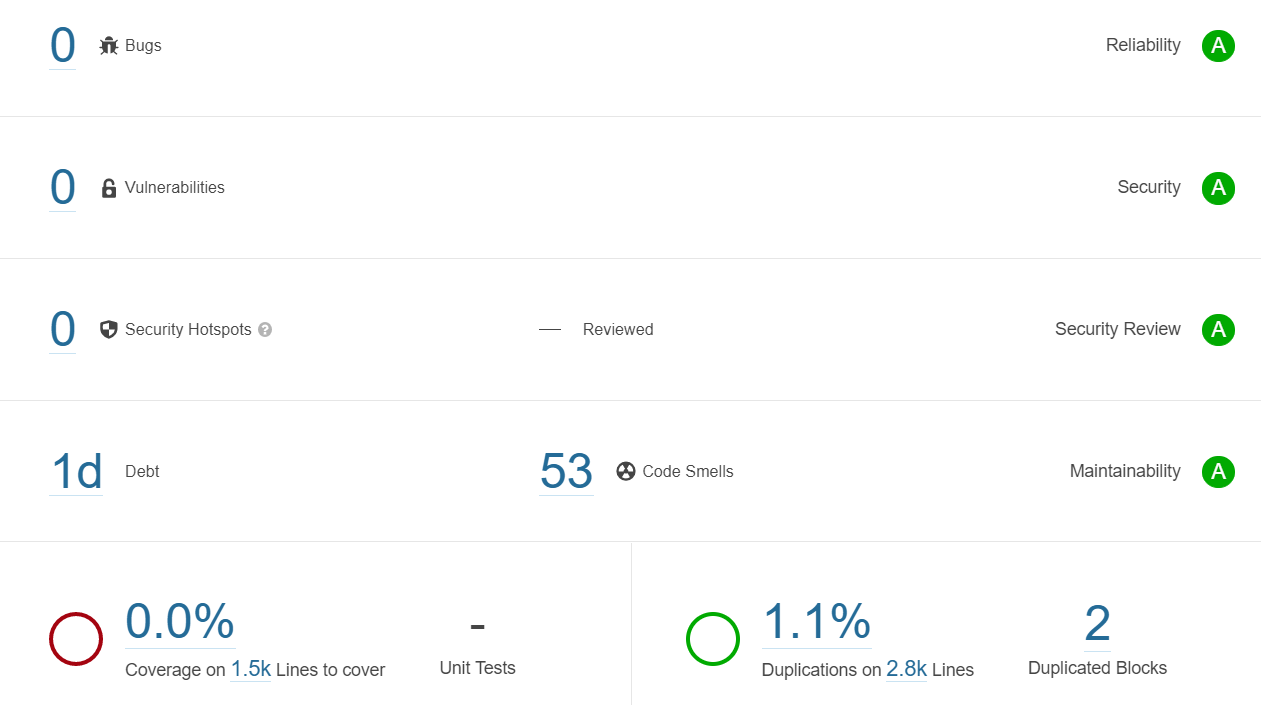
\includegraphics[scale=0.60]{Immagini/form/Sonarqube.png}
\\\\
Sono stati individuati e corretti i principali issue presenti nel codice.
Non è stato possibile rimuovere i code smells rimanenti in quanto sono parte integrante della struttura del codice e rimuoverli avrebbe richiesto un completo refactor del progetto.
\end{document}